% Outras Opções:
%   * openright  -- Força início de capítulos em páginas ímpares (padrão da
%                   biblioteca)
%   * oneside    -- Desliga frente-e-verso
%   * nominatalocal -- Lê os dados da nominata do arquivo nominatalocal.def
\documentclass[ppgc,diss,english,openright]{iiufrgs}

\usepackage[utf8]{inputenc}
\usepackage[alf,abnt-emphasize=bf]{abntex2cite}	% pacote para usar citações abnt

\usepackage{lmodern}
\usepackage{amsmath}
\usepackage{amsthm}
\usepackage{enumitem}
\usepackage{listings}
\usepackage{xcolor}
\usepackage{amsfonts}
\usepackage{newtxtext,newtxmath}
\usepackage{semantic}
\usepackage{float}
\usepackage{mdframed}
\usepackage{stmaryrd}
\usepackage{multicol}
\usepackage{graphicx}
\usepackage{todonotes}
\usepackage{mathtools}
\usepackage{etoolbox}
\usepackage[normalem]{ulem}
\usepackage{fontawesome}

\usepackage{times}
\usepackage{palatino}
\usepackage[all,knot,arc,import,poly]{xy}

\usepackage{tikz,tkz-euclide}
\usetikzlibrary{backgrounds,calc,shapes,shapes.geometric}
%\usepackage{subfig}
\usepackage{caption}
\usepackage{subcaption}
\captionsetup[subfigure]{justification=centering}

\usepackage{pdfpages}

\usepackage{wasysym}
\usepackage{minted}

%For todo notes, remove in final version
\setlength{\marginparwidth}{2cm}
\newcommand{\tinytodo}[2][]
{\todo[caption={#2}, size=\footnotesize, #1]{\renewcommand{\baselinestretch}{0.5}\selectfont#2\par}}

\newcommand{\critical}[1]{\todo[color=red]{\textbf{Critical:} #1}}
\newcommand{\important}[1]{\textcolor{red}{\textbf{\texttt{#1}}}}
%\newcommand{\newadd}[1]{\uline{#1}}
\newcommand{\newadd}[1]{#1}

\theoremstyle{plain}
\newtheorem{thm}{Theorem}[chapter]

\theoremstyle{definition}
\newtheorem{definition}[thm]{Definition}
\newtheorem{example}[thm]{Example}
\newtheorem{assumption}[thm]{Assumption}
\newtheorem*{remark}{Remark}
\newtheorem*{notation}{Notation}
\AtEndEnvironment{definition}{\hfill\qedsymbol}%put \null before \hfill?
\AtEndEnvironment{assumption}{\hfill\qedsymbol}
\AtEndEnvironment{remark}{\hfill\qedsymbol}
\AtEndEnvironment{notation}{\hfill\qedsymbol}
\AtEndEnvironment{example}{\hfill$\blacksquare$}

\def\changemargin#1#2{\list{}{\rightmargin#2\leftmargin#1}\item[]}
\let\endchangemargin=\endlist

\newenvironment{intuition}{\begin{changemargin}{1cm}{1cm}}{\end{changemargin}}

%% Diagram commands
\newcommand{\diagram}[1]{\centerline{\xymatrix{#1}}}
\newcommand{\parens}[1]{\left(#1\right)}
\newcommand{\morph}[3]{\mbox{${#1} : {#2} \rightarrow {#3}$}}

%% Graph Grammars constructions
\newcommand{\graphrule}{\mbox{$p = \left(L \xleftarrow{l} K \xrightarrow{r} R\right)$}}
\newcommand{\ruleone}{\mbox{$p_1 = \left(L_1 \leftarrow K_1 \rightarrow R_1\right)$}}
\newcommand{\ruletwo}{\mbox{$p_2 = \left(L_2 \leftarrow K_2 \rightarrow R_2\right)$}}
\newcommand{\inversegraphrule}{\mbox{$p^{-1} = \left(R \xleftarrow{r} K \xrightarrow{l} L\right)$}}
\newcommand{\lefthand}{\mbox{$l : K \rightarrow L$}}
\newcommand{\righthand}{\mbox{$r : K \rightarrow R$}}
\newcommand{\nac}{\mbox{$n : L \rightarrow N$}}
\newcommand{\nacone}{\mbox{$n_1 : L_1 \rightarrow N_1$}}
\newcommand{\nactwo}{\mbox{$n_2 : L_2 \rightarrow N_2$}}
\newcommand{\rightnac}{\mbox{$n : R \rightarrow N$}}
\newcommand{\match}{\mbox{$m : L \rightarrow G$}}
\newcommand{\comatch}{\mbox{$m' : R \rightarrow H$}}
\newcommand{\rulesequence}{\mbox{$p_0,\ldots,p_{n-1},p_n$}}
\newcommand{\graphGrammar}{\mbox{$GG = \left(TG,I,P\right)$}}

%% Doubly-typed Graph Gramars constructions
\newcommand{\doublyTypedGraph}{\mbox{$G^{TG^{T}}$}}
\newcommand{\doublyTypedRule}{\mbox{$p^{TG^T} = \left(L^{TG^T} \leftarrow K^{TG^T} \rightarrow R^{TG^T}\right)$}}
\newcommand{\inverseDoublyTypedRule}{\mbox{$\parens{p^{TG^T}}^{-1} = \left(R^{TG^T} \leftarrow K^{TG^T} \rightarrow L^{TG^T}\right)$}}
\newcommand{\doublyTypedGraphGrammar}{\mbox{$GG = \left(TG^T, I^{TG^T},P \right)$}}
\newcommand{\doublyTypedGraphGrammarCore}{\mbox{\ensuremath{GG = \left(C^T, I^{C^T},P \right)}}}
\newcommand{\occurrenceGrammar}{\mbox{\ensuremath{OGG = \left(C^T, I^{C^T},A \right)}}}
\newcommand{\coreGraph}{\ensuremath{C^T}}
\newcommand{\action}{\mbox{$a = \left(L_a \xleftarrow{l} K_a \xrightarrow{r} R_a, L_a \xrightarrow{n_i} [N_i]\right)$}}
\newcommand{\initialGraph}{\mbox{\ensuremath{I^{\coreGraph}}}}

%% Category Constructions
\newcommand{\cat}[1]{\mbox{\ensuremath{\mathbf{#1}}}}
\newcommand{\typedGraphCategory}{\cat{TGraph_T}}
\newcommand{\doublyTypedGraphCategory}{\cat{DTGraph_{TG^T}}}

\newcommand{\code}[1]{\texttt{#1}}
\newcommand{\hide}[1]{}

\newcounter{doubly-typed-grammar-counter}
\addtocounter{doubly-typed-grammar-counter}{0}


% avoid LaTeX Font Warning: Font shape `U/stmry/b/n' undefined
\SetSymbolFont{stmry}{bold}{U}{stmry}{m}{n}

\title{Occurrence Graph Grammars with Negative Application Conditions}
\author{Santos Bezerra}{Jonas}
\advisor[Prof$^a$.]{Ribeiro}{Leila}
%\date{maio}{2001}
\location{Porto Alegre}{RS}

% itens individuais da nominata podem ser redefinidos com os comandos
% abaixo:
% \renewcommand{\nominataReit}{Prof\textsuperscript{a}.~Wrana Maria Panizzi}
% \renewcommand{\nominataReitname}{Reitora}
% \renewcommand{\nominataPRE}{Prof.~Jos{\'e} Carlos Ferraz Hennemann}
% \renewcommand{\nominataPREname}{Pr{\'o}-Reitor de Ensino}
% \renewcommand{\nominataPRAPG}{Prof\textsuperscript{a}.~Joc{\'e}lia Grazia}
% \renewcommand{\nominataPRAPGname}{Pr{\'o}-Reitora Adjunta de P{\'o}s-Gradua{\c{c}}{\~a}o}
% \renewcommand{\nominataDir}{Prof.~Philippe Olivier Alexandre Navaux}
% \renewcommand{\nominataDirname}{Diretor do Instituto de Inform{\'a}tica}
% \renewcommand{\nominataCoord}{Prof.~Carlos Alberto Heuser}
% \renewcommand{\nominataCoordname}{Coordenador do PPGC}
% \renewcommand{\nominataBibchefe}{Beatriz Regina Bastos Haro}
% \renewcommand{\nominataBibchefename}{Bibliotec{\'a}ria-chefe do Instituto de Inform{\'a}tica}
% \renewcommand{\nominataChefeINA}{Prof.~Jos{\'e} Valdeni de Lima}
% \renewcommand{\nominataChefeINAname}{Chefe do \deptINA}
% \renewcommand{\nominataChefeINT}{Prof.~Leila Ribeiro}
% \renewcommand{\nominataChefeINTname}{Chefe do \deptINT}

\keyword{Graph Grammars}
\keyword{Occurrence Graph Grammars}
\keyword{Negative Aplication Conditions}
\keyword{Semantics}

\newcommand{\pu}{processing unit}
\newcommand{\Pu}{Processing unit}
\newcommand{\pus}{processing units}
\newcommand{\Pus}{Processing units}
\newcommand{\envid}{env_{id}}

\definecolor{kwcolor}{rgb}{0,0.5,0}
\definecolor{bgcolor}{rgb}{0.98, 0.98, 0.98}
\definecolor{numbercolor}{rgb}{0.1,0.1,0.1}

\lstset{
  keywordstyle=\bfseries\underbar,
  stringstyle=\itshape,
  basicstyle=\small\ttfamily,
  frame=bt,
  framerule=1pt,
  numbers=left,
  numbersep=10pt,
  numberstyle=\scriptsize\color{numbercolor},
  backgroundcolor=\color{bgcolor},
  tabsize=2
}

\lstdefinelanguage{l1}
{keywords={let, letrec, in, if, then, else, end, unused}%
  sensitive=true,
  alsoletter={\$},
  comment=[l]{\#},
  string=[b]"
}

\lstdefinelanguage{acqua-ir}
{keywords={unused, EnvNew, EnvAdd, Call, unused}%
  sensitive=true,
  alsoletter={\$},
  comment=[l]{\#},
  string=[b]"
}

\graphicspath{ {images/} }
%\captionsetup[table]{skip=10pt}
\newmdenv[leftline=false,rightline=false]{openframe}



\captionsetup[figure]{position=below,labelfont=bf}
\captionsetup[subfigure]{position=bottom}
\sloppy
\begin{document}

\hide{ Template for code snippets
\begin{figure}[!ht]
\caption{Colimit Implementation}
\begin{minted}[linenos=true, breaklines,fontsize=\small]{haskell}
\end{minted}
\label{fig:tests-colimit}
\end{figure}
}

\maketitle
\clearpage

% dedicatoria
\clearpage
\begin{flushright}
  \mbox{}\vfill
  {\sffamily\itshape
  ``Poste, kiam \^si pripensis la aferon,\\
  \^si opiniis ke tio ja estis mirinda,\\
  sed kiam \^gi okazis \^cio \^sajnis tute natura.''\\}
  --- \textsc{Alico en Mirlando}
\end{flushright}

% agradecimentos
\chapter*{Acknowledgement}
  I'm very happy with everything I've accomplished so far and although I still have a long way to go, I must thank some amazing people in my life without whom this path would be a lot harder, if not impossible.

  First of all, I would like to thank Prof. Leila Ribeiro for giving me the opportunity to work with her even without previously knowing me: You are such an inspiring advisor and working with you always made me feel like I can improve myself and push me to the next level. Working with you was, at the same time, very challenging and joyful. I also need to thank professors Rodrigo Machado, Érika Cota and Lúcio Duarte, for always being there for conversations and feedback about this work, you were really a great help.

  I owe a very special thank you to Calebe and Marília, for helping me settle in Porto Alegre when I knew nothing, nowhere and nobody here. You guys really made my life a lot easier.

  To Andrei, Guilherme, Leonardo and Ana, my colleagues and friends, it was both an honour and a pleasure to work and live with you. I will always cherish our memories together as some of my favourites. To all the guys from lab 202, Diego, Fabi, Marcelo, Marina, Marlo, Felipe Tanus, Michele, Felipe Grando, Jéssica e Pedro: we need to go out more. To my very first friends in Porto Alegre, Shauna and Maurício, thank you for all the good moments. 

  To my old friends, Wendell, Gabriel, Malu and Jéssica, who were always by my side despite the 3178km of distance, your constant contact and kindness helped me through a lot of critical moments. I love you guys.

  Ao meu irmão, Mateus, com quem eu sei que sempre posso contar e por quem eu sempre tentei dar o melhor de mim, de tal forma que ele tenha tanto orgulho de quem eu sou e da família que formamos: obrigado por me aceitar como eu sou.
  
  Finalmente, para mainha, Dona Necila... eu jamais poderei expressar suficientemente o quão a senhora foi importante em todas as minhas conquistas até agora. A senhora sempre foi a pessoa que mais admiro na vida, por toda sua luta, dedicação e sacrifícios para dar a mim e aos meus irmãos todas as oportunidades que a senhora não teve. Esse mestrado é tão seu quanto meu. Vou te amar pra sempre.

\begin{abstract}
    Graph Grammars are based on the application of rules that are able to modify graphs, as such, they provide a suitable formalism to model complex systems in an intuitive and precise manner, providing both a graphical language and a solid formal background for systems analysis. Therefore, they have been used in a wide range of applications within Computer Science, specially in the field of Model-Driven Development.
    Particularly, the study of the Semantics of Graph Grammars, i.e. which graphs belong to the language of a grammar and which derivations are possible within the context of a grammar, provides a powerful framework for reasoning about the execution behaviour of systems modelled as Graph Grammars.
    There are several different ways of specifying the Semantics of Graph Grammars.
    One notable possibility is the use of Occurrence Graph Grammars, which encodes the Semantics in a structure that is also a Graph Grammar itself. Occurrence Graph Grammars differ from other semantic models such as Unfolding and Canonical Derivations mainly by providing a more compact, easier to analyse structure. They were introduced in the nineties and used ever since, however the original definitions lack the inclusion of Negative Application Conditions, additional structures imposed over the rules of a grammar to better tune their possible applications according to the execution context.
    Given the important role Negative Application Conditions play in the modelling and analysis of complex systems as Graph Grammars nowadays, this thesis presents an extension of the framework of Occurrence Graph Grammars to include them. It also presents its implementation in Verigraph, a system specification and verification tool based on graph rewriting.
\end{abstract}

\begin{englishabstract}{Gramáticas de Grafos de Ocorrência com Condições Negativas de Aplicação}{Gramáticas de Grafos. Gramáticas de Grafos de Ocorrência. Condições Negativas de Aplicação. Semântica}
  Gramáticas de Grafos baseiam-se na aplicação de regras que modificam grafos, fornecendo assim um formalismo adequado para a modelagem de sistemas complexos de forma intuitiva e precisa, além de fornecer uma notação gráfica descomplicada e uma base formal sólida para a análise de sistemas. Dados tais atributos, essas gramáticas possuem uma ampla gama de aplicações dentro da Ciência da Computação, especialmente no campo do Desenvolvimento Orientado a Modelos. Particularmente, o estudo da semântica de
  Gramáticas de Grafos (isto é, quais grafos pertencem à linguagem da gramática e quais derivações são permitidas no contexto da gramática) provê uma poderosa ferramenta para compreender e analisar o comportamento de sistemas modelados como Gramáticas de Grafos. Existem diversas formas de especificar a semântica de Gramáticas de Grafos, uma delas é o uso de Gramáticas de Grafos de Ocorrência que codificam tal semântica em estruturas que também são, por sua vez, Gramáticas de Grafos. Gramáticas de
  Grafos de Ocorrência foram introduzidas nos anos noventa e utilizadas desde então, porém as definições originais não incluem o uso de Condições Negativas de Aplicação, estruturas adicionais anexadas às regras de uma gramática para refinar as possíveis aplicações das regras em determinados contextos. Dada a atual importância das Condições Negativas de Aplicação na modelagem de sistemas complexos, essa dissertação propõe uma extensão da teoria das Gramáticas de Grafos de Ocorrência de forma a
  incluí-las, além de apresentar a implementação desta teoria no Verigraph, uma ferramenta de especificação e verificação de sistemas baseada em reescrita de grafos.
\end{englishabstract}


\begin{listofabbrv}{SPMD}
   \item[DPO] Double Pushout
   \item[GG] Graph Grammar
   \item[GTS] Graph Transformation System
   \item[GUI] Graphical User Interface
   \item[NAC] Negative Application Condition
%   \item[NC] Negative Atomic Constraint
   \item[OGG] Occurrence Graph Grammar
%   \item[PB] Pullback
%   \item[PC] Positive Atomic Constraint
   \item[PO] Pushout
   \item[SPO] Single Pushout
\end{listofabbrv}

%  \begin{listofsymbols}{$\alpha\beta\pi\omega$}
%         \item[$\leftarrow$] Morphism
%  \end{listofsymbols}

\listoffigures
\tableofcontents

\chapter{Introduction}

Graph grammars are a suitable formalism to model complex systems in an intuitive and precise manner, providing both a graphical straightforward language and a solid formal background for system analysis. In this framework, (computational) system states are modelled as graphs, while transitions between different states are modelled as graph transformation rules. By using them it is possible to simulate the execution of a modelled system and also analyse several properties about its behaviour, such as termination, concurrency, reachable states, among others~\cite{Ehrig2006}. Among the analysis techniques provided by graph grammars, we have:

\begin{itemize}
  \item Critical Pairs and Critical Sequences Analyzes; the first one allows us to verify which rules conflict (i.e. prohibit) the application of another and why; the second, which rules depend on the execution of others to be applied and why~\cite{Lambers2008a}; 
  \item Calculation of Concurrent Rules; which summarizes the results of applying several different rules in only one rule; 
  \item State Space Exploration and Model Checking; \important{complete}
  \item Unfolding, Graph Processes and Canonical Derivations; \important{complete}
\end{itemize}

\important{[Small, trivial examples to easy the explanation]}

Given such properties, graph grammars have found a wide range of applications within Computer Science, specially in the field of model-driven software development, where the transformation of visual models is a vital part of the process and additionally a natural application of graph grammars~\cite{Rozenberg1997}. As proof of such suitability, several non-trivial systems have been modelled and studied under the optics of graph grammars, such as telephone communications~\cite{Ribeiro1996}, elevator and railroad control~\cite{Lambers2010, Pennemann2009} and integration of service-oriented systems~\cite{Giese2015}, to cite just a few.

Besides its powerful applications, the use of graph grammars as a framework for modelling systems provides us with a great advantage over other formalisms: it makes possible for non-specialists in the field to generate graph grammar models of a system and still benefit from the rigorous analyzes it offers. For example, ~\cite{Junior2015,BezerraWEIT2016,Cota2017} explain how to generate graph grammars from a set of textual requirement documents such as use cases, functional specifications and other kinds of guidelines by means of a systematic methodology. They also present guidance towards using different graph grammars analysis techniques in order to improve and verify these documents and, therefore, the systems they describe.

In this work, we are concerned about the semantics of graph grammars\ldots

\important{Graph grammars and their semantics}

\important{What is the semantics of a graph grammar?}

\important{Why is it important?}

\important{How can it be obtained using Occurrence Graph Grammars}

We believe that the use of graph grammars as a model for the generation of test cases and oracles may improve the reliability of the testing activity by using the solid formal semantics of the formalism, while requiring little theoretical expertise from the user. The main objective of this thesis can be summarized as follows:

\begin{intuition}
  \center{\textit{Given the graph grammar model of a software system, how can a set of relevant test cases and oracles be generated for the system?}}
\end{intuition}\hfill\break

Where by \emph{relevant} we mean (1) a set of test oracles capable of deciding, for any input, which paths of execution and which states of the system are valid: \textbf{verifiability}; (2) a set of tests covering all as many flows of execution as feasible: \textbf{coverage}; while (3) tests avoid repetition of equivalent paths: \textbf{compactness}.

The concepts and ideas developed during this work will also be implemented in Verigraph~\cite{verigraph,Costa2016}, a new system for specification and verification of software that is based on graph grammars and category theory.

\important{Explain better that we are generating tests for graph grammars: more theory, less software engineering.}

\newadd{The main contributions of this thesis are (1) the development of a computer-aided strategy for the generation of test cases from graph grammars, which required (2) an extension of the Occurrence Graph Grammar framework in order to allow the tests generation for complex, realistic systems modelled as graph grammars. Finally, (3) the implementation of this strategy in the Verigraph System.}

\hfill \break
\textbf{Structure of the Thesis:}

\begin{description}
  \item[Chapter~\ref{ch:gts}:] In this chapter we review the basic notions of graph transformation systems, specifically under the Double-Pushout (DPO) approach, as well as the notions of parallel and sequential independency of rules.

  \item[Chapter~\ref{ch:process}:] In this chapter we present an overview of doubly-typed graph grammars and other constructions necessary to accomplish occurrence graph grammars. Also, how these occurrence grammars can be used to represent the concurrent semantics of their original grammar.

    We also present out extension to previous works in occurrence graph grammars to include the notion of negative application conditions, which is part of our thesis contribution.

  \item[Chapter~\ref{ch:verigraph}:] This chapter presents an overview of the Verigraph system, which was used to implement implement the techniques presented in this thesis. Verigraph in itself represents a novelty in the field of graph transformations, being the first tool implemented in a functional language, which favored its source code to be very close to the problem domain itself.

  \item[Chapter~\ref{ch:tests}:] This chapter briefly reviews a methodology to extract graph grammar models from the use use cases of a system. Furthermore, we provide a strategy to extract test cases from calculated occurrence graph grammars, which is implemented in Verigraph, and argue about the relevance of the generated set of tests.

  \item[Chapter~\ref{ch:conclusions}:] This chapter presents some related work, then summarizes our results and presents our conclusions. Moreover, it shows remaining open problems and future work.

  \item[Appendix~\ref{app:category-theory}:] This appendix contains a brief introduction to category theory and the categorial constructions used in this thesis.

  \item[Appendix~\ref{app:tutorial}:] This appendix contains the Verigraph manual, explaining in the details how the system can be downloaded, installed and used.

  \item[Appendix~\ref{app:use-cases}] This appendix contains the use cases and modelled graph grammar used as case study on section~\ref{ch:tests}.
\end{description}

\chapter{Graph Grammars}

\section{Overview of Graph Transformation, definitions, algorithms, etc.}

\begin{intuition}
\end{intuition}

\begin{mydef}{Graph}
\end{mydef}

\begin{mydef}{Graph Morphism}
\end{mydef}

\begin{mydef}{Typed Graph}
\end{mydef}

\begin{mydef}{Typed Graph Morphism}
\end{mydef}

% Should I put the definitions of Graphs, Typed Graphs and its morphisms?

\begin{mydef}{Graph Production}
\end{mydef}

\begin{mydef}{Atomic Constraints}

\diagram{
  P\ar[rr]^{a}\ar[dr]_{p} & & C\ar[dl]^{q}\\
  & G &
}

\end{mydef}

\begin{mydef}{Negative Application Condition}

\diagram{
  N\ar@{.>}[dr]|{| q} & L\ar[d]^{m}\ar[l]_{n}\\
   & G
}

\end{mydef}

\begin{mydef}{Graph Transformation System}
\end{mydef}

\begin{mydef}{Graph Grammar}
\end{mydef}

\begin{mydef}{Parallel and Sequential Independence}
\end{mydef}


\section{Occurence Graph Grammars}

\begin{mydef}{Doubly-Typed Graph}
\end{mydef}

\begin{mydef}{Doubly-Typed Graph Morphisms}
\end{mydef}

\begin{mydef}{Doubly-Typed Graph Grammars}
\end{mydef}

\begin{mydef}{Core Graph}
\end{mydef}

%\chapter{Concurrent Rules}

\section{Motivation}

What kind of concurrent rule do we expect and why?

\section{Concurrent Rules}

\begin{definition}{Downward Shifted NACs}

\diagram{
  N'_j\ar@{.>}@/0.5pc/[r]^{e_{ji}} & N_i\ar@{}[dl]|{=}\\
  A\ar[r]_{m}\ar[u]^{n'_j} & B\ar[u]_{n_i}
}

For each $NAC(n'_j)$ on $A$ with $n'_j : A \rightarrow N'_j$ and $m : A \rightarrow B$, 
let $D_m(NAC(n'_j)) = \{ NAC(n_i)|i \in I, n_i : B \rightarrow N_i \}$ where $I$ and $n_i$ 
are constructed as follows:
\begin{itemize}
  \item $i \in I$ iff $(e_{ji}, n_i)$ with $e_{ji} : N'_j \rightarrow N_i$ jointly surjective 
  \item $e_{ji} \circ n_i = n_i \circ m$
  \item $e_{ji}$ injective
\end{itemize}

For each set of NACs $NAC_A = {NAC(N_j)| j \in J}$ on $A$ the downward shift of $NAC_A$ is then defined as: $D_m(NAC_A) = \cup_{j \in J}D_m(NAC(n'_j))$. $D_m$ is also called the \emph{Downward shift of $NAC_A$}.

\end{definition}

\begin{definition}{Left NACs from Right NACs}

\centerline{\xymatrix{
  L\ar[d]_{n'_i} & K\ar[l]\ar[r]\ar[d] & R\ar[d]^{n_i}\\
  N'_i\ar@{}[ur]|{(2)} & D\ar[l]\ar[r] & N_i\ar@{}[ul]|{(1)}
}}

\end{definition}

\begin{definition}{Conflicts and Dependencies}
\end{definition}

\begin{definition}{Concurrent Rules with NACs}

A concurrent rule is
\end{definition}

\centerline{
\xymatrix{
  N_i & & & & N_j & & \\
  L_c\ar[d]\ar[u]^{n_i}\ar@{}[dr]|{(3)} & K_c\ar[d]\ar[l]\ar[r] \ar@{}[dr]|{(1)} & R_c\ar[dr]^{e_1} & & L_n\ar[dl]_{e_2}\ar[u]^{n_j} & K_n\ar[d]\ar[l]\ar[r]\ar@{}[dl]|{(2)} & R_n\ar[d]\ar@{}[dl]|{(4)}\\
  L & C_c\ar[l]^{c_l}\ar[rr]_{c_r} & & \textit{E} & & C_n\ar[ll]^{n_l}\ar[r]_{n_r} & R\\
  & & & K\ar@{.>}@/1pc/[llu]^{k_c}\ar@{.>}@/1pc/[urr]_{k_n}\ar@{}[u]|{(5)} & & &
}}

\begin{itemize}
\item $n = 0$ The \emph{concurrent rule} $p_c$ with NACs for rule $p_0$ with NACs is $p_0$ with NACs itself.
\item $n \geqslant 1$ A concurrent rule $p_c = p'_c \ast_E p_n $ with NACs for the rule sequence \rulesequence is defined recursively as $p_c = (l_c \circ k_c : K \rightarrow L, r_n \circ k_n : K \rightarrow R)$ where 
  \begin{itemize}
  \item $p'_c : L'_c \leftarrow K'_c \rightarrow R'_c$ is a concurrent rule for the sequence $p_0,\ldots,p_{n-1}$
  \item $(e'_c,e_n)$ is jointly surjective
  \item (1), (2), (3) and (4) are pushouts
  \item (5) is a pullback
  \item $N_i$ is shifted over morphism $l'$
  \item $N_j$ is shifted over morphism $e_2$ and then over the ``rule'' $q'_c = l_c : C_c \rightarrow L, r_c : C_c \rightarrow E$
  \end{itemize}
\end{itemize}

\begin{definition}{Concurrent Rules induced by Dependencies}

  \textbf{incomplete}

\diagram{
  N_i& & & & N_j\ar@{.>}@/_3pc/[ddllll]_{e_2} & & \\
  L_c\ar[u]^{n_i}\ar[d]_{e_1}\ar@{}[dr]|{(1)} & K_c\ar[d]\ar[l]\ar[r] \ar@{}[dr]|{(2)} & R_c\ar[dr]^{m'_1} & & L_n\ar[dl]_{m_2}\ar[u]^{n_j} & K_n\ar[d]\ar[l]\ar[r]\ar@{}[dl]|{(3)} & R_n\ar[d]^{m'_2}\ar@{}[dl]|{(4)}\\
  \textit{E} & C_c\ar[l]|{c_l}\ar[rr]|{c_r} & & P_1 & & C_n\ar[ll]|{n_l}\ar[r]|{n_r} & P_2\\
  & & & K\ar@{.>}@/1pc/[llu]|{k_c}\ar@{.>}@/1pc/[urr]|{k_n}\ar@{}[u]|{(5)} & & & 
}

\end{definition}
% \ar@{.>}@/_1pc/[dlll]|{X_{h_{21}}}

\begin{thm}{EpiPairs}
  \begin{proof}{Incomplete}
  \end{proof}
\end{thm}

\subsection{Inapplicable concurrent rules}

\begin{definition}{Rules with trivially triggered NACs}
\end{definition}

\begin{thm}{Propagation of trivially triggered NACs over concurrent rules}
  \begin{proof}{Yet to come}
  \end{proof}
\end{thm}

\begin{definition}{Breaking constraint rules}
\end{definition}

\chapter{Occurrence Graph Grammars with NACs}\label{ch:process}

Occurrence Graph Grammars (OGGs) were defined for the Single-Pushout (SPO) approach by~\cite{Ribeiro1996}, and for the Double-Pushout (DPO) approach by~\cite{Corradini1996}. In both cases they consist of a way of representing the concurrent semantics of a graph grammar as a graph grammar itself.

  The aim of an OGG is to describe all possible states and changes of states of the graph grammar from which it was constructed.
  This is possible because occurrence grammars can be regarded as an execution history of the underlying grammar.
  This history is encoded under the forms of (1) a \emph{core graph} containing all elements ever used in the execution of the grammar, (2) a set of \emph{actions}, which are rule applications typed over this core graph and (3) a set of \emph{relations} between these actions and the elements of the core graph.

  These relations express dependencies among core graph elements, such as which of them must occur together, at the same state, which ones must be created/deleted one after the other, which elements must never occur together, and so on.
  They also encode restrictions over the application of rules, such as which rules are sequentially dependent on others or whether it is possible to successfully apply all the rules of a grammar, etc.
  %This property makes occurrence graph grammars excellent candidates for the generation of test cases, as we are interested in a way of representing several (equivalent) possible derivations using a compact notation.

  However, Negative Application Conditions are not addressed by the original definitions of occurrence grammars.
    Still, NACs are nowadays essential for modelling complex systems as graph grammars, given they provide more compact mechanisms to control the application of rules~\cite{Habel1996, Lambers2008, Corradini2014}.
      In this chapter, after reviewing the works of~\cite{Ribeiro1996} and~\cite{Corradini1996} in OGGs, an extension of the occurrence grammars framework towards contemplating negative application conditions is presented, which is part of our thesis contribution.

\section{Occurrence Graph Grammars with NACs}

\begin{definition}[Doubly-Typed Graph] Given a type graph $T$, a \emph{doubly-typed graph} \doublyTypedGraph{} over $T$ is a tuple \doublyTypedGraph $= \left(G^T,TG^T, t^{G^T} : G^T \rightarrow TG^T\right)$ where $G^T$ and $TG^T$ are typed graphs over $T$ and \mbox{$t^{G^T} : G^T \rightarrow TG^T$} is a typed graph morphism in \typedGraphCategory{}. We call $TG^T$ the \emph{double-type graph} and $t^{G^T}$ the double-typing morphism.
\end{definition}

\begin{remark}[Typing Morphism] As we are interested in occurrence graph grammars, we consider only doubly-typed graphs whose typing morphism $type_{TG} : TG \rightarrow T$ is an epimorphism. This has the effect that every element present in $T$ is the image of at least one element from $TG$.
\end{remark}

\begin{example}[Doubly-Typed Graph Example] Figure~\ref{fig:process:doubly-typed-graph} shows a doubly-typed graph $G^{TG^T}$.
\end{example}

\begin{figure}[!ht]
  \centering
  \fbox{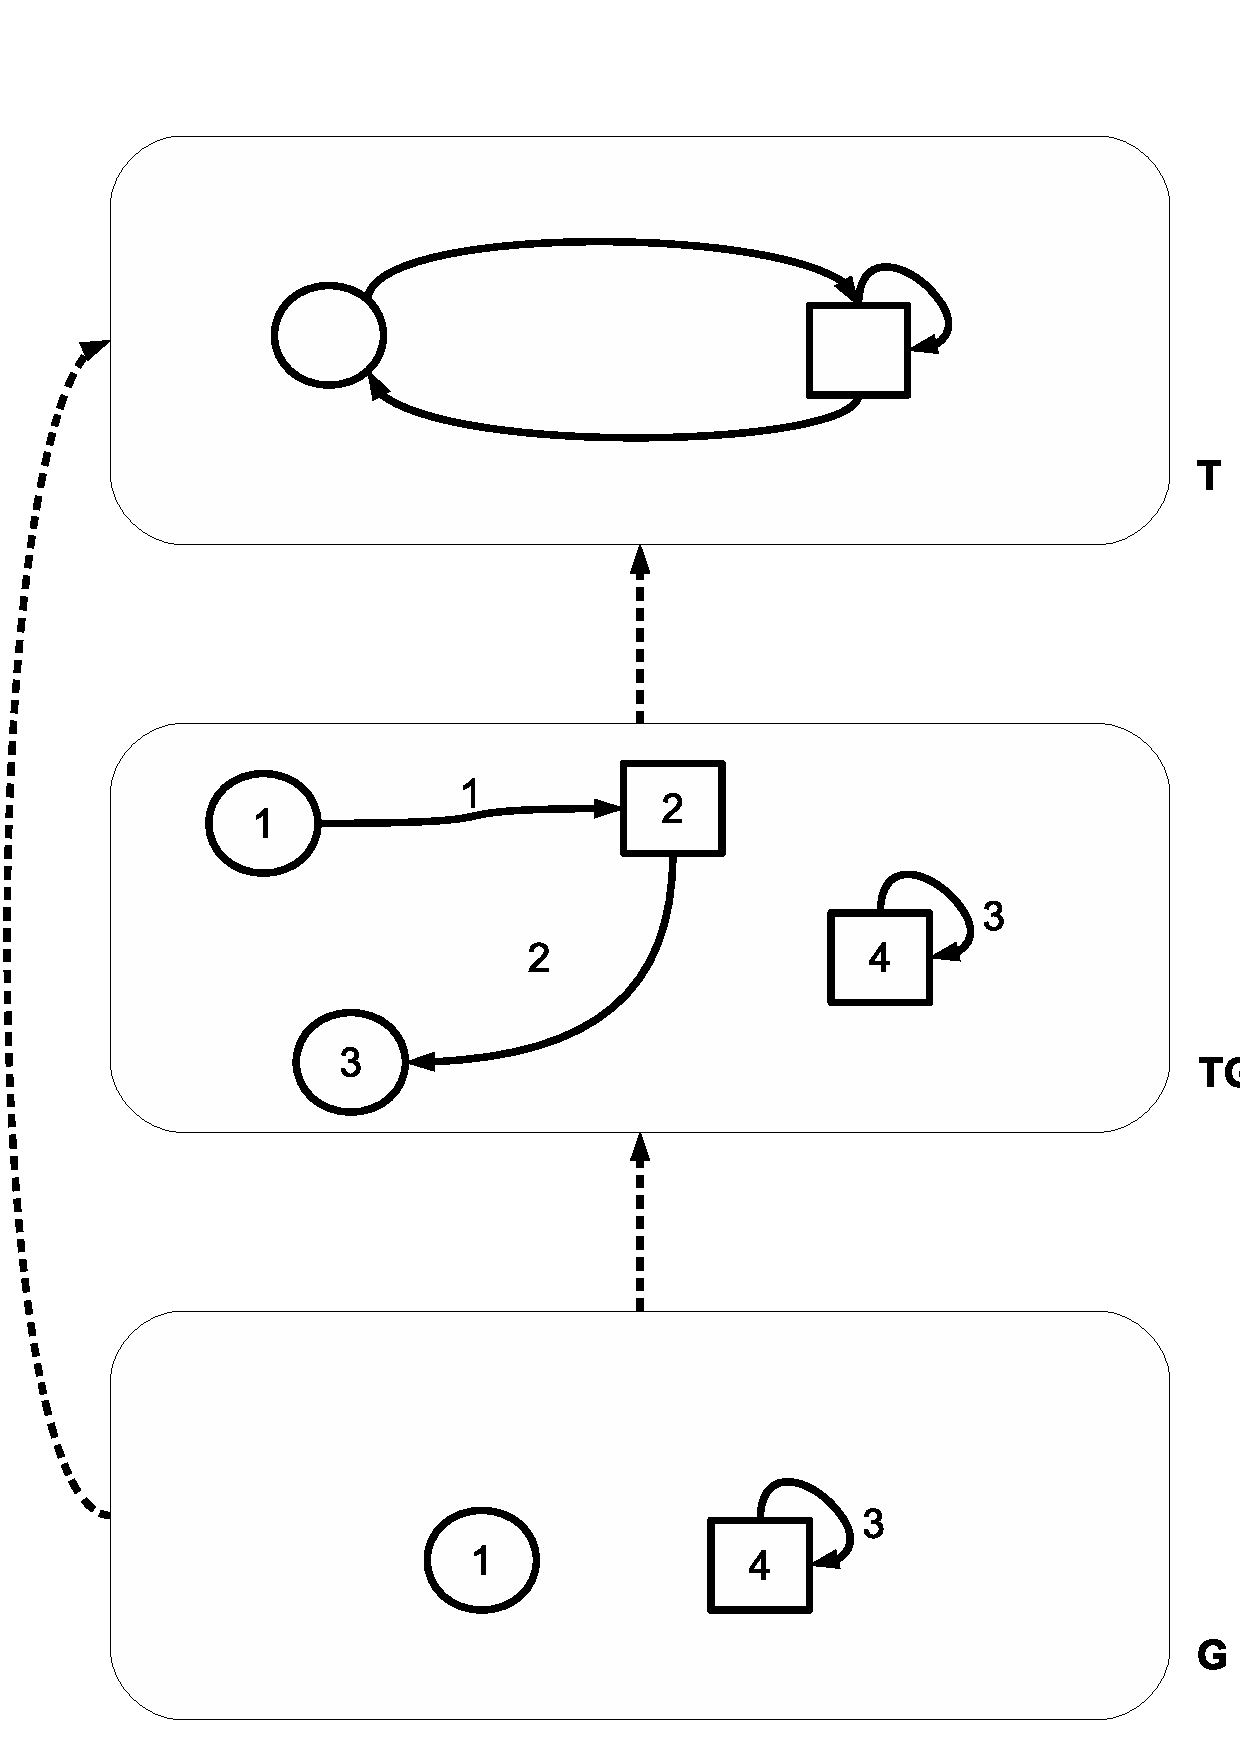
\includegraphics[scale=0.6]{images/process/doubly-typed-graph-example}}
  \caption{Doubly-typed graph}\label{fig:process:doubly-typed-graph}
\end{figure}

\begin{definition}[Doubly-Typed Graph Morphism]
  Given two doubly-typed graphs $G^{TG^T}$ and $H^{TG^T}$ and a graph morphism $g^T : G^T \rightarrow H^T$, we say that $g^T$ is a \emph{$TG^T$-doubly-typed graph morphism} if the following diagram commutes:

\diagram{
  G\ar[rr]^{g}\ar[dr]_{t^{G}}& & H\ar[dl]^{t^{H}} \\
   & TG\ar[d]^{type_{TG}} & \\
  & T &
}
\end{definition}

Notice that the (single) type morphisms $type_G : G \rightarrow T$ and $type_H : H \rightarrow T$ can be obtained respectively as $type_{TG} \circ t^G$ and $type_{TG} \circ t^H$.

\begin{example}[Doubly-Typed Graph Morphism Example] Figure~\ref{fig:process:doubly-typed-graph-morphism} shows a doubly-typed graph morphism $f : G^{TG^T} \rightarrow H^{TG^T}$.
\end{example}

\begin{figure}[!ht]
  \centering
  \fbox{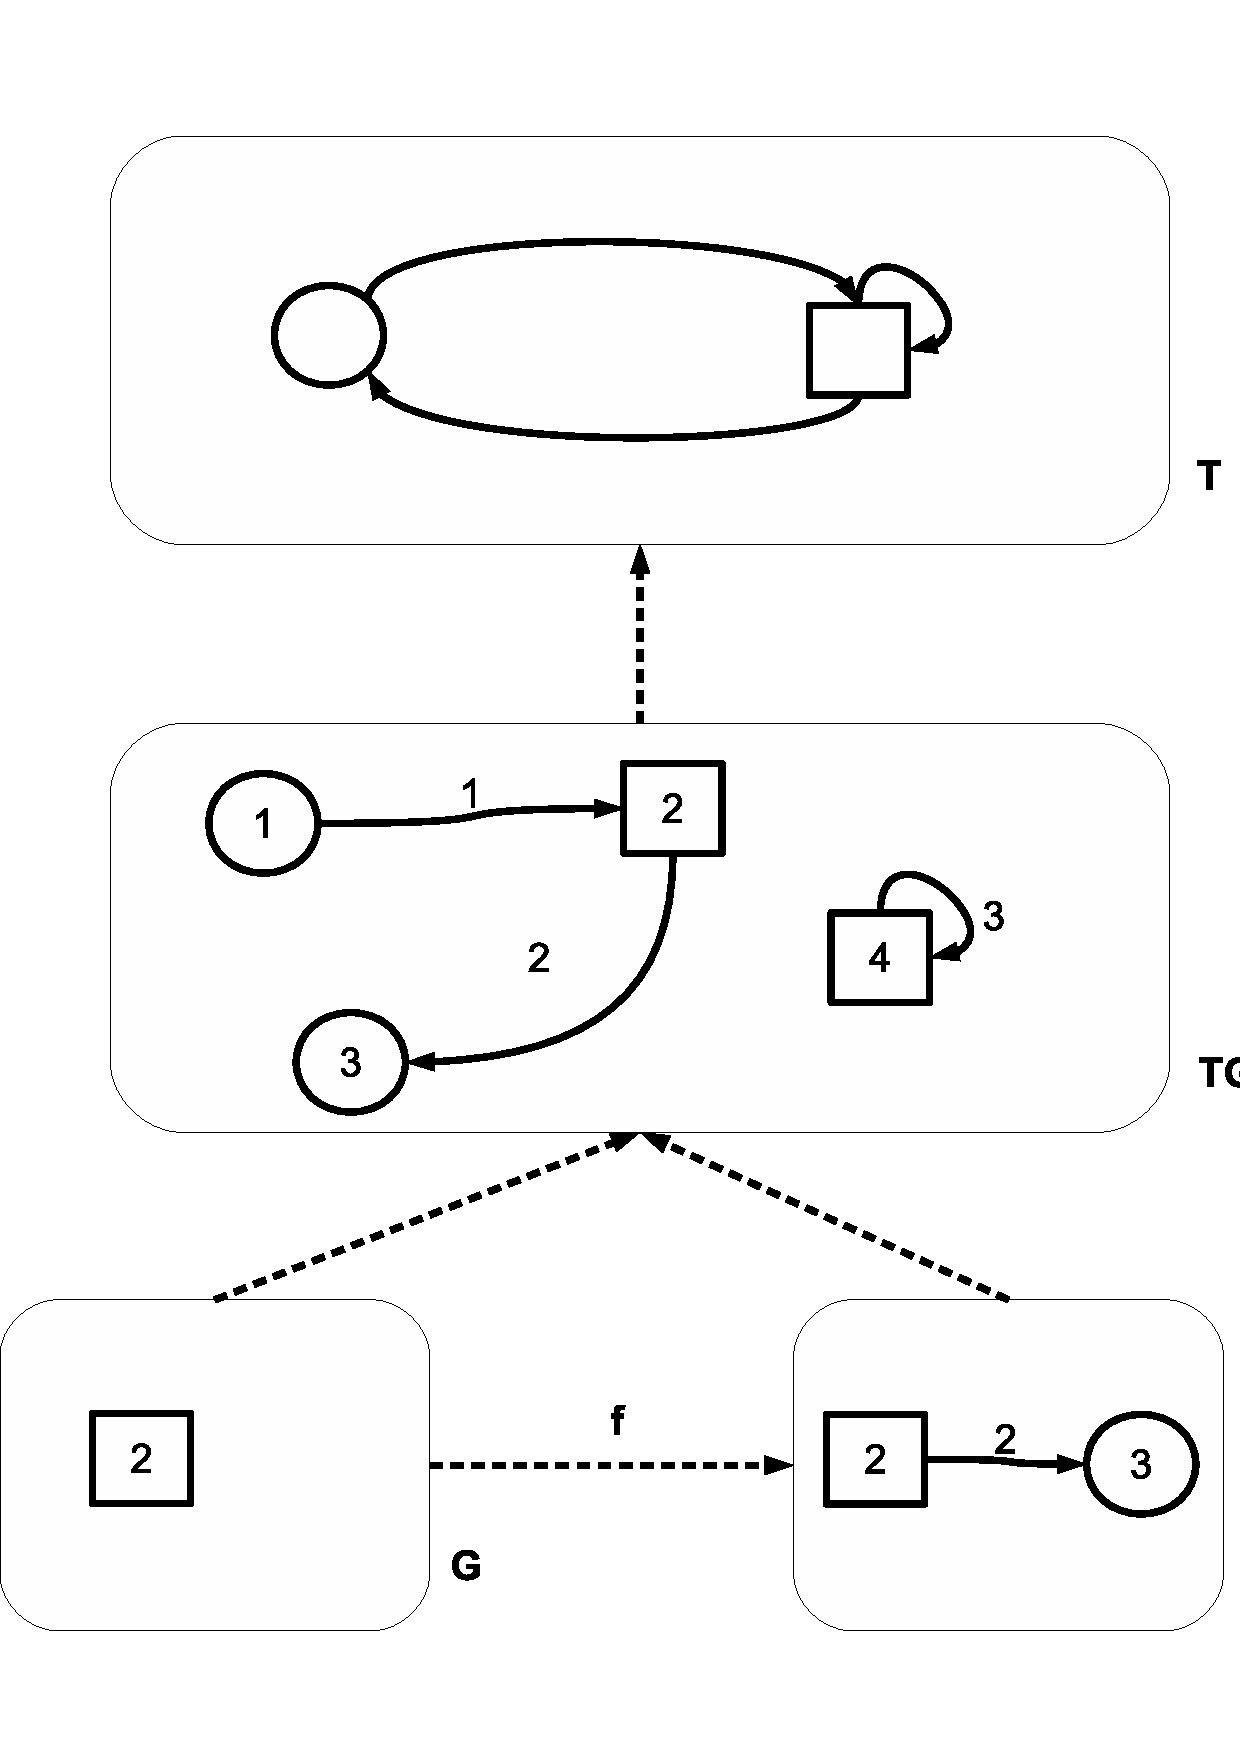
\includegraphics[scale=0.6]{images/process/doubly-typed-graph-morphism-example}}
  \caption{Doubly-typed graph morphism}\label{fig:process:doubly-typed-graph-morphism}
\end{figure}

\begin{remark} \cite{Ribeiro1996} defined different kinds of doubly-typed graph morphisms based on whether the double-type graphs and the type graphs are or are not the same. In this work we are only interested in the case where all doubly-typed graphs share exactly the same double-type and type graphs. Therefore, through the rest of this work, we refer to \mbox{\emph{$TG^T$-doubly-typed graph morphisms}} simply by \emph{doubly-typed graph morphisms}.
\end{remark}


\begin{definition}[Doubly-Typed Graph Rule] A doubly-typed graph rule \doublyTypedRule{} is a span of injective doubly-typed graph morphisms $l : K \rightarrow L$ and $r : K \rightarrow R$.

\diagram{
  L\ar[dr] & K\ar[l]\ar[r]\ar[d] & R\ar[dl]\\
    & TG\ar[d] & \\
    & T &
}

  Given a doubly-typed graph rule \doublyTypedRule{}, its inverse rule is defined by \inverseDoublyTypedRule{}.

  Let the double-typing morphisms from $L^{TG^T}$, $K^{TG^T}$ and $R^{TG^T}$ be $t^{L^T}$, $t^{K^T}$ and $t^{R^T}$, respectively. For a rule $a = p^{TG^T}$ we call:

  \begin{itemize}
    \item $L_a = L_T$, $K_a = K_R$ and $R_a = R_T$, the left, gluing and right graphs of $a$.
    \item $pre_a = t^{L^T} : L^T \rightarrow TG^T$, the \emph{pre-condition} of the $a$.
    \item $post_a = t^{R^T} : R^T \rightarrow TG^T$, the \emph{post-condition} of $a$.
    %\item $r_a = r^T$, the \emph{rule pattern} of $a$.\tinytodo{Not sure if we will need the rule pattern.}
  \end{itemize}
\end{definition}

\begin{example}[Doubly-Typed Graph Rule Example]Figure~\ref{fig:process:doubly-typed-graph-rule} shows a doubly-typed graph rule which deletes an edge $\curvearrowleft_1$ and a node $\Circle_1$, preserves a $\Square_2$ and creates a node $\Circle_3$ and an edge $\curvearrowleft_2$.
\end{example}

\begin{figure}[!ht]
  \centering
  \fbox{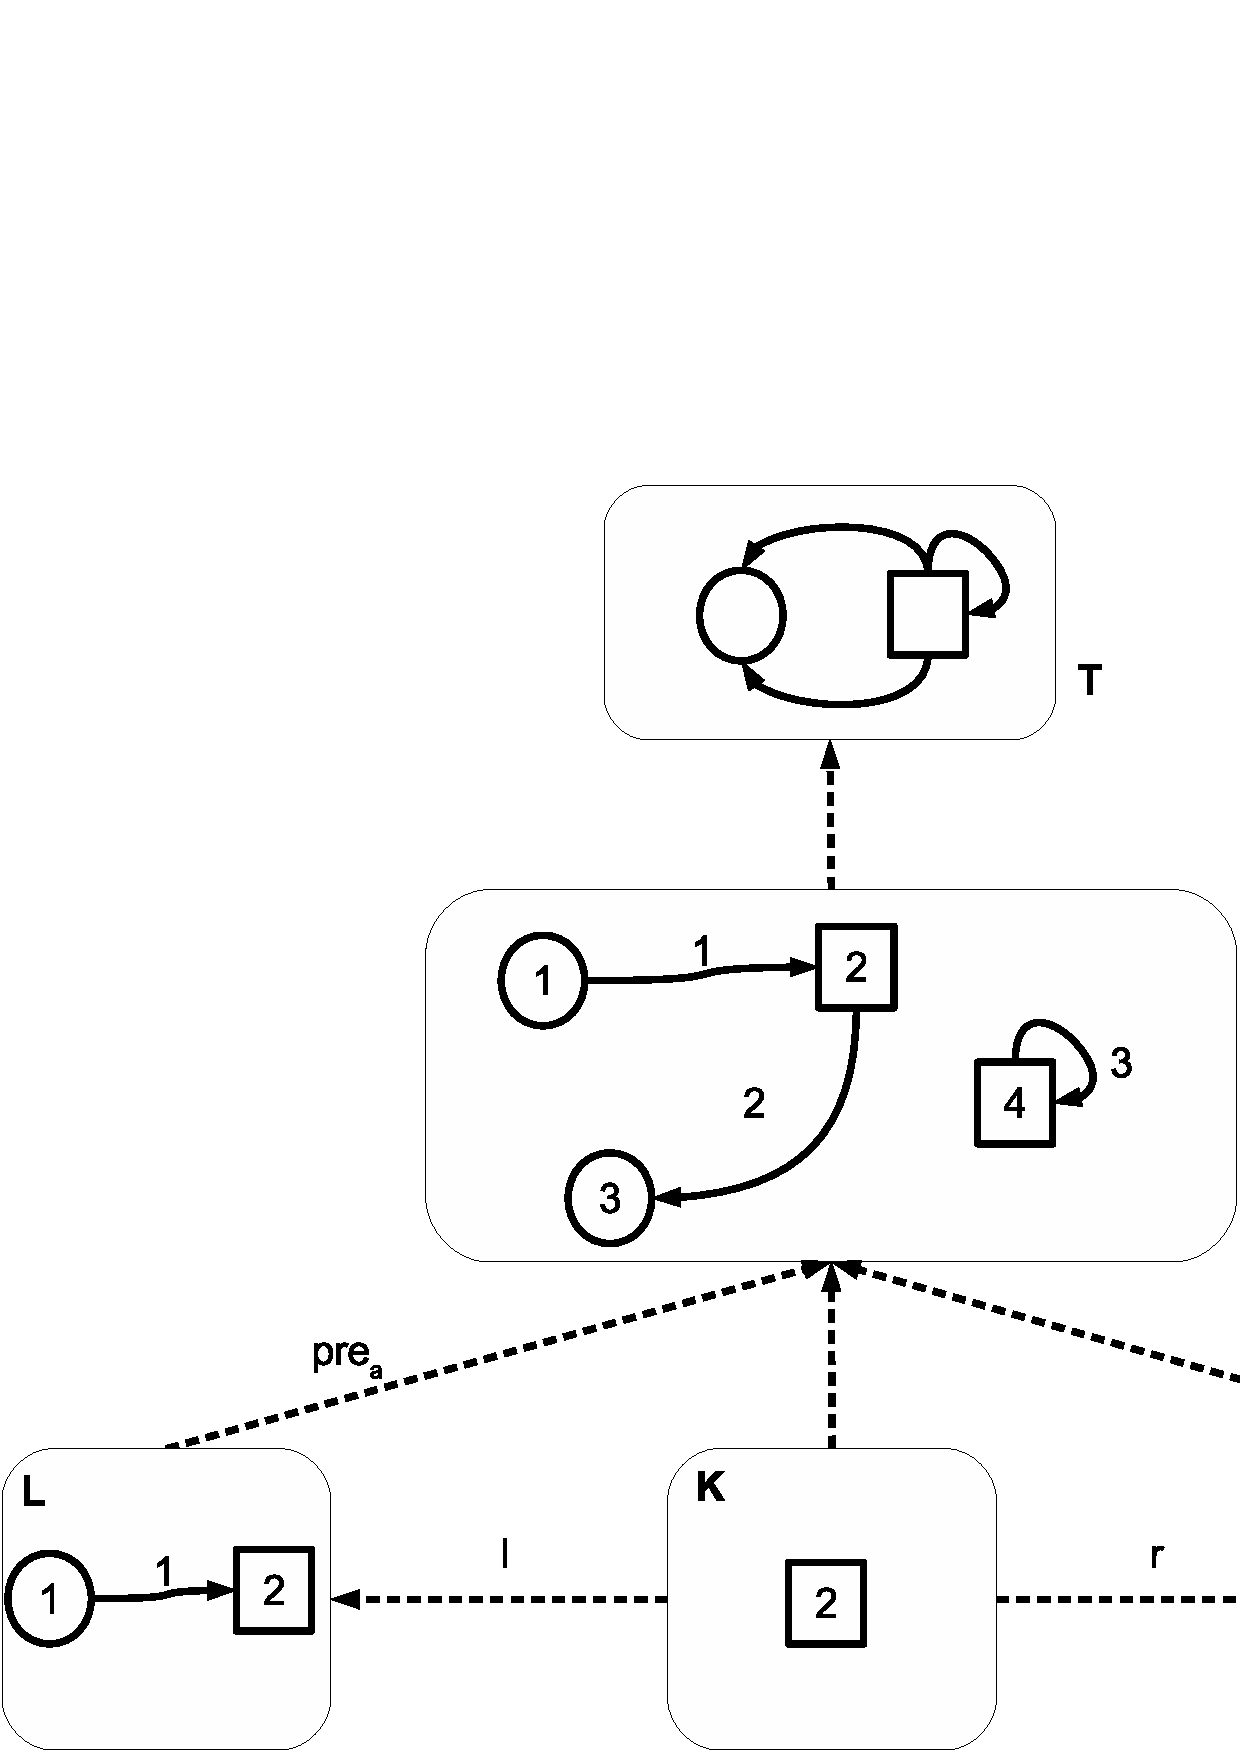
\includegraphics[scale=0.5]{images/process/doubly-typed-graph-rule-example}}
  \caption{Doubly-typed graph rule}\label{fig:process:doubly-typed-graph-rule}
\end{figure}

\begin{definition}[Negative Application Conditions on Doubly-Typed Graph Rules] A \emph{left} negative application condition over a doubly-typed graph rule $p^{TG^T}$ is of the form $NAC(n^T)$, where $n^T : L^T \rightarrow N^T$ is an arbitrary (single-)typed graph morphism. 
 
A (doubly-typed) match morphism $m^{TG^T} : L^{TG^T} \rightarrow G^{TG^T}$ of a rule $p^{TG^T}$ satisfies $NAC(n^T)$ on $L^{TG^T}$, written \mbox{$m^T \models NAC(n^T)$}, iff $\nexists$ $q^T : N^T \rightarrow G^T$ where $q^T$ injective and $q^T \circ n^T = m^T$.

\diagram{
  T & TG\ar[l]\\
  N\ar[u]\ar@{.>}[dr]|{|}_{q} & L\ar[u]\ar[d]^{m}\ar[l]_{n}\\
   & G\ar@/_2.1pc/[uu]
}

  A match $m^{TG^T} : L^{TG^T} \rightarrow G^{TG^T}$ satisfies a set \mbox{$NAC_L = \{NAC\left(n^T_i\right)|i \in I\}$} of left $NACs$, iff \mbox{$m \models NAC\left(n^T_i\right)$} $\forall i \in I$.

\emph{Right} negative application conditions are defined analogously for the right hand side of a rule and its comatch.
\end{definition}

\begin{remark}
  We could have defined NACs whose morphisms are doubly-typed graph morphisms, which would then act specifically over doubly-typed graphs. However, the use of this kind of NAC could lead to a doubly-typed grammar with a set of NACs much bigger than the original one, thus we do not use this kind of NACs given our interest in a compact and more abstract characterization for the semantics of graph grammars. Therefore, we use \emph{single-typed} NACs as the only NAC type in all of our \emph{doubly-typed graph grammars}, and $NAC(n)$ as a synonym of $NAC(n^T)$.
\end{remark}

In a grammar without NACs, if there is a sequence of graph transformations $t_0\ldots t_n$ where each pair $(t_i,t_{i+1})$ of consecutive transformations is sequentially independent, then it is possible to \emph{switch} the
order of application for any pair in that sequence an arbitrary number of times and still achieve the same final graph as a result (up to isomorphism). This property is called \emph{switch equivalence}~\cite{Corradini2013}.

However, the switch equivalence does not always hold when the grammar has NACs. This happens because there may be situations where the NAC of a rule can be triggered by the cumulative effect of applying two (or more) other rules, while the same rules would not trigger that NAC in isolation. This may lead to a situation where conflicts and dependencies
	are not \emph{stable under switch}, which means that conflicts or dependencies that do not occur in a given sequence of transformations may arise if one or more pairs of transformations are switched. An example is shown in Figure~\ref{ex:process:instability}.

\begin{example}[Switch Equivalence]\label{ex:process:instability}The rules depicted in Figure~\ref{fig:process:instability} show a situation where the independence between rules is not stable under switch equivalence.

  In this example, all rules are independent and also do not conflict with each other in the sense of Definitions~\ref{def:classic-dependency} and~\ref{def:classic-conflict}. 
  Thus, in theory, it should be possible to apply these rules in any order or in parallel. Particularly, it may be possible to apply all rules in the order they appear in the figure: $[p_1, p_2, p_3]$. 
  It may also be possible to apply them in the orders $[p_1, p_3, p_2]$, $[p_2, p_1, p_3]$ and $[p_3, p_1, p_2]$. 
  However, it is not possible to perform a derivation using the rules in the orders $[p_2, p_3, p_1]$ or $[p_3, p_2, p_1]$. This problem arises from the fact that $p_2$ and $p_3$ independently create a piece of the pattern forbidden by the NAC of $p_1$ in a way that, although the effect of each rule by itself does not trigger the NAC of $p_1$, their combined effects do.
\end{example}

\begin{figure}[!ht]
  \centering
  \fbox{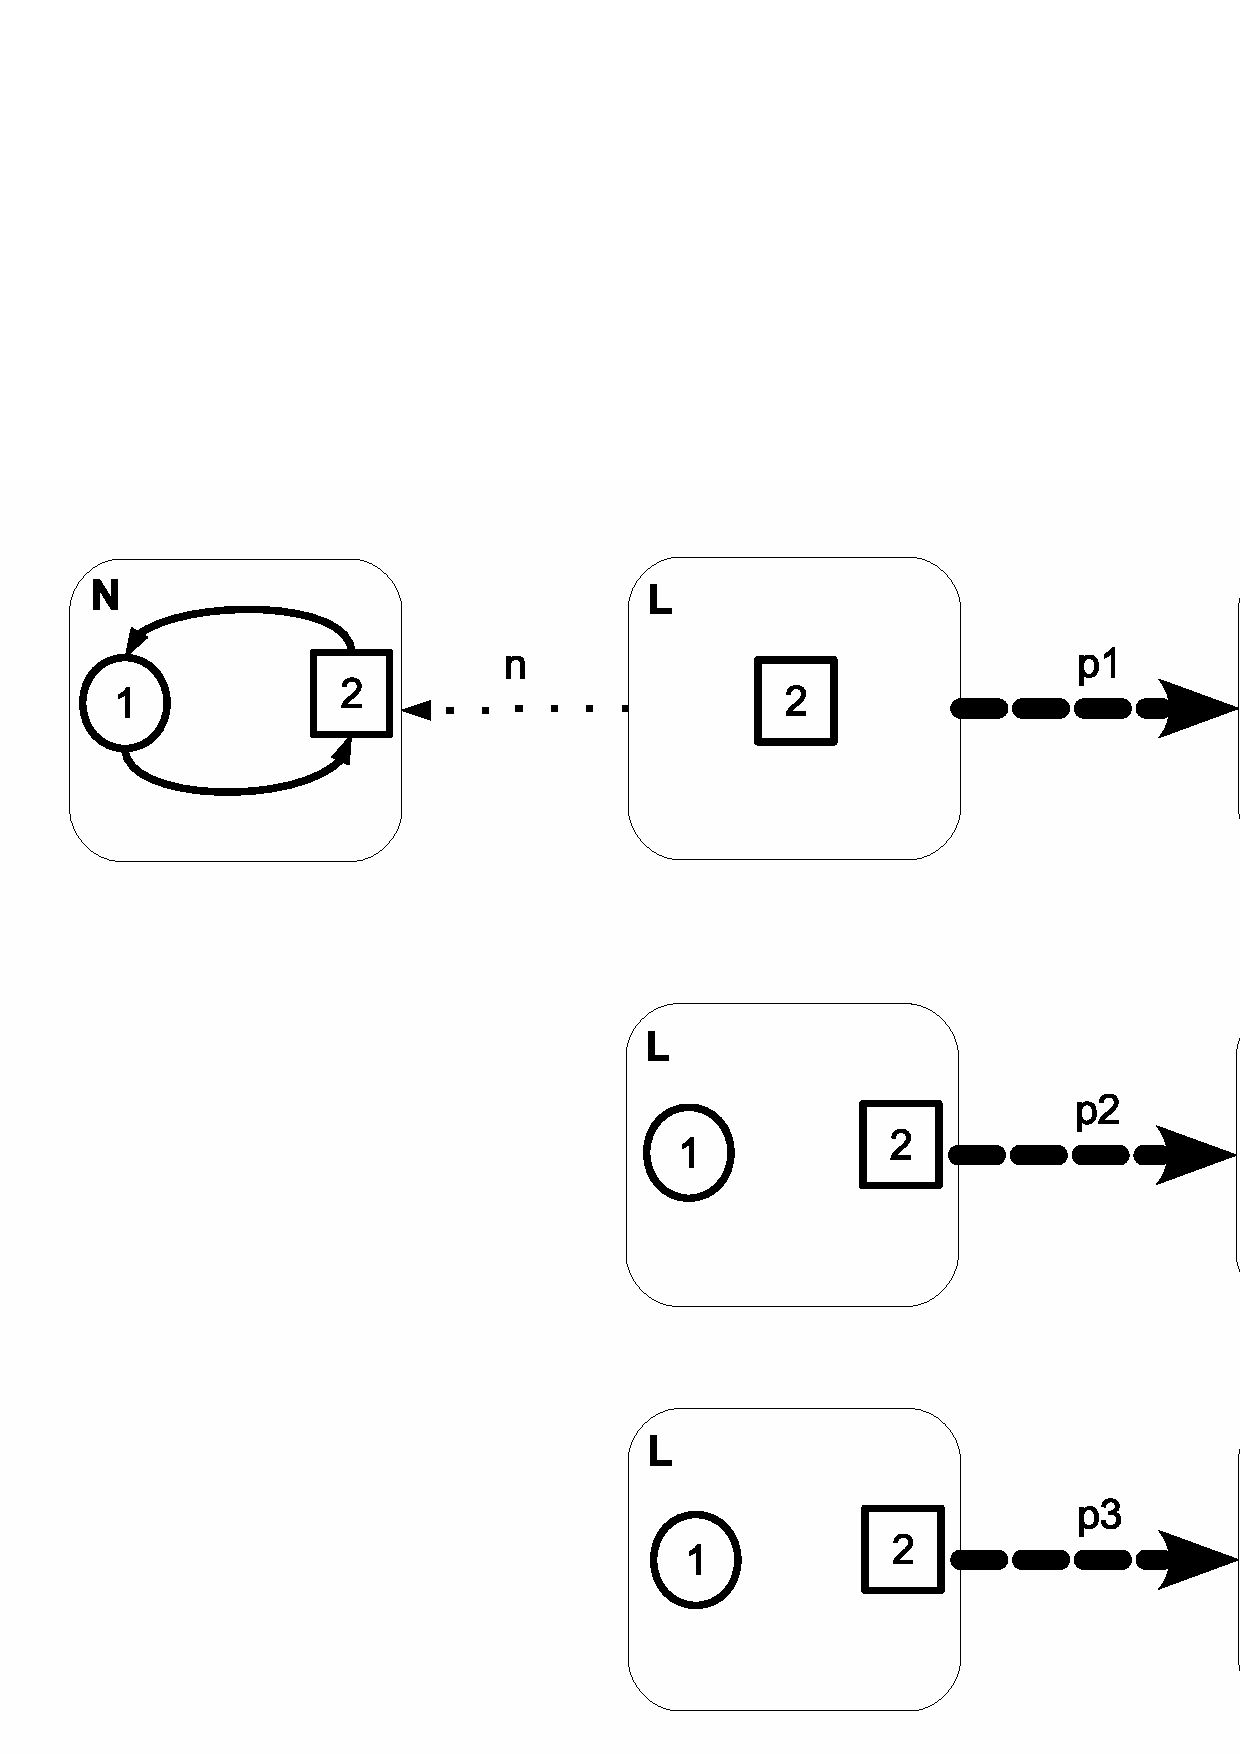
\includegraphics[scale=0.5]{images/process/instability-example}}
  \caption{Instability of conflicts under shift\\}\label{fig:process:instability}
\end{figure}

In order to avoid this problem while we construct a canonical representation of several possible derivations for a set of rules, we restrict the use of NACs to a special type of NACs called \emph{incremental NACs}.
\emph{Incremental NACs} were originally defined in~\cite{Corradini2013} and~\cite{Corradini2014}. They have the property of extending the forbidden context of a match by a single edge or a single node. Thus, each NAC forbids only one element at a time and therefore there is no possible way to trigger a NAC by the cumulative effects of more than one rule.

\begin{definition}[Incremental NACs] Given a monomorphism \mbox{$n : L \rightarrow N$}, $NAC(n)$ is said to be incremental if for any possible pair of decompositions \mbox{$g_1 : L \rightarrow O_g;g_2 : O_g \rightarrow N$} and \mbox{$f_1 : L \rightarrow O_f;f_2 : O_f \rightarrow N$} as in the diagram below, where all morphisms are monos and \mbox{$f_1;f_2 = n = g_1;g_2$}, there exists a mediating morphism $o_1 : O_g \rightarrow O_f$ or $o_2 : O_f \rightarrow O_g$, such that the resulting triangles
  commutes.

\diagram{
  & O_g\ar[dr]^{g_2}\ar@{.>}@/_0.5pc/[dd]|<<<<<<{o_1} &  \\
  L\ar[ur]^{g_1}\ar[dr]_{f_1}\ar[rr]|<<<<{n}&     & N\\
    & O_f\ar[ur]_{f_2}\ar@{.>}@/_0.5pc/[uu]|<<<<<<<<{o_2} & 
}

\end{definition}

\begin{example}[Incremental NACs]Figure~\ref{fig:process:incremental-nacs} shows all possible (canonical) formats that any valid incremental NAC may assume.

\begin{figure}[!ht]
  \centering
  \fbox{\includegraphics[scale=0.7]{images/process/incremental-nacs}}
  \caption{Canonical Incremental NACs}\label{fig:process:incremental-nacs}
\end{figure}
\end{example}

At first, it may seem that we are loosing expressive power by restricting the NACs used in our grammars to incremental NACs only. However ~\cite{Corradini2013} have shown two important results regarding them. First, they showed that incremental NACs are sufficient to model most of real applications using $GTS$s. Second, they presented an algorithm to compile rules with general NACs to rules with incremental NACs only, generating a new $GTS$ that is able to simulate the original one.

  \begin{notation}[Set Operations over Graphs] Given a graph $G$, we sometimes view them as being composed of a set $V(G)$ of nodes and a set $E(G)$ of edges, denoted \mbox{$G = V(G) \cup E(G)$}, in order to allow the use of set operations over this graph.
    For example, we say that an element (a node or an edge) $x$ is a member of $G$, denoted $x \in G$, iff $x \in V(G) \cup E(G)$. 
      Moreover, any operations involving multiple graphs are applied \emph{setwise}. For example, given two graphs $G_1$ and $G_2$, the difference $D = G_1 - G_2$ between them is the union of the differences between their sets of nodes and their sets of edges. Therefore $D = V(D) \cup E(D)$ where $V(D) = V(G_1) - V(G_2)$ and $E(D) = E(G_1) - E(G_2)$.

    Any other set operations applied over graphs are regarded likewise.
%\mbox{$D = G_1 - G_2 = V(G_1) \cup E(G_1) - V(G_2) \cup E(V_2) = (V(G_1) - V(G_2)) \cup (E(G_1) - E(G_2))$}

\end{notation}

\begin{definition}[Triggering element] Given a rule \graphrule{} with an incremental, non trivially triggered NAC \nac{}, and a monomorphic match \match{}, where there is an injective $q : N \rightarrow G$, therefore $m \not\models NAC(n)$. There is exactly one element that completes the match towards triggering the NAC, this element is present in the difference between the images of $q$ and $m$.

  Let $G_{|N}$ be the image of $q$, $G_{|L}$ the image of $m$, and \mbox{$D = G_{|N} - G_{|L}$}. The triggering element of this NAC is:

  \begin{itemize}
    \item $x \in E(D)$, if $E(D) \neq \varnothing$;
    \item $x \in V(D)$ otherwise.
  \end{itemize} 
\end{definition}

\begin{example}[Triggering Element]
  Given that incremental NACs extend the match by forbidding only one element at a time, this element can be easily identified at the instance graph: it corresponds to the solely element mapped by the morphism \morph{q}{N}{G} which is not also mapped by \morph{m}{L}{G}. Figure~\ref{fig:process:triggering-element} shows an example. The elements in the instance graph mapped by either $q$ or $m$ are represented by dashed lines. Notice that the only element which is not in the image of
  both morphisms is $\curvearrowleft_2$, therefore $\curvearrowleft_2$ is the triggering element of the NAC for this match.
\end{example}

\begin{figure}[!ht]
  \centering
  \fbox{\includegraphics[scale=0.7]{images/process/triggering-element}}
  \caption{Triggering Element}\label{fig:process:triggering-element}
\end{figure}

\begin{definition}[Doubly-Typed Graph Grammars] A \emph{doubly-typed graph grammar} is a tuple $GG = \left(TG^T, I^{TG^T},P \right)$ where $TG^T$ is the double-type graph of the grammar, $I^{TG^T}$ is a doubly-typed graph called the \emph{initial graph} and $P$ is a set of doubly-typed graph rules.

\end{definition}


\begin{definition}[Core Graph]\label{def:core-graph} Given a doubly-typed graph grammar \doublyTypedGraphGrammarCore{}, we have that \coreGraph{} is a \emph{core graph} iff the following two conditions hold:

\begin{description}

  \item[(uniqueness of origin)] \mbox{$\forall x \in$ \coreGraph $: \exists! y \in (I^T \uplus (\uplus_{i \in P} (R_i - K_i))$}:
\[ x =
    \begin{cases}
      in_{GG}\parens{y},$ if $y \in I^T\\
      post_i(y),$ if $y \in R_i - K_i\\
    \end{cases}
   \]

 \item[(uniqueness of deletion)] \mbox{$\forall x \in$ \coreGraph $: \exists^{\leq1} y \in \uplus_{i \in P} (L_i - K_i)$}:
\[ x =
    \begin{cases}
      pre_i(y),$ if $y \in L_i - K_i\\
    \end{cases}
   \]\end{description}

\end{definition}
  The first condition assures that every element in the \emph{core graph} was either already present in the initial graph or was created by one and only one rule. The second condition assures that for every element that is deleted, it is deleted only once by only one rule. The idea is that each element within a \emph{core graph} has a unique origin. At the same time, the \emph{core graph} contains all elements necessary (created, deleted and preserved) by all rules in its underlying grammar. 
  
  In~\cite{Ribeiro1996} the second condition was not used, because of a peculiarity of the SPO approach where more than one rule can delete the same element at the same time, while this would raise a conflict and therefore be forbidden in the DPO approach. As a consequence, the occurrence grammars defined by~\cite{Ribeiro1996} are inherently non-deterministic, whereas ours are deterministic.  In practice, this means that the semantics of a graph grammar in the SPO approach can be achieved with only one occurrence grammar, while in the DPO approach we need a set of them.

\begin{example}[Doubly-Typed Graph Grammar and Core Graph Example] \mbox{Figure~\ref{fig:process:core-graph:counter-example}} shows a doubly-typed graph grammar, whose double-type is not a core graph. That happens because $\Square_2$ is created by both rules $p_1$ and $p_2$, as well as $\Circle_1$ is deleted by both $p_2$ and $p_3$.

  On the other hand, Figure~\ref{fig:process:core-graph:example} shows a doubly-typed graph grammar whose double-type is also a core graph: $\Square_2$ and $\curvearrowleft_1$ are created by $p_1$, $\curvearrowleft_3$ by $p_2$, $\Circle_3$ and $\curvearrowleft_2$ by $p_3$ and $\Circle_1$ is present on the initial graph. Also, the deleted elements are deleted only once: $\Circle_1$ and
  $\curvearrowleft_1$ by $p_3$.

  It is important to notice that, even though the $TG$ graphs in both grammars are isomorphic, only the one in Figure~\ref{fig:process:core-graph:example} is a core graph. This can be explained by looking to their underlying grammars (initial graphs and rules), where one of them satisfies the conditions presented in Definition~\ref{def:core-graph} while the other does not.
\begin{figure}[!ht]
  \centering
  \begin{subfigure}[t]{.5\textwidth}
    \centerline{\fbox{\includegraphics[scale=0.5]{images/process/core_graph/counter_example}}}
    \caption{A grammar with a double-type graph that is not a core graph.}\label{fig:process:core-graph:counter-example}
  \end{subfigure}
  \begin{subfigure}[t]{.5\textwidth}
    \centerline{\fbox{\includegraphics[scale=0.5]{images/process/core_graph/example}}}
    \caption{A grammar with a double-type graph that is also a core graph.}\label{fig:process:core-graph:example}
  \end{subfigure}

  \caption{Doubly-typed graph grammars}\label{fig:process:doubly-typed-grammars}
\end{figure}

\end{example}

\begin{notation}[Restriction to Image] Given an arbitrary morphism $f : A \rightarrow X$, we denote as $f' : A \rightarrow X_{|A}$ the morphism derived from $f$ where $X_{|A}$ is the image of $f$.

  For two arbitrary morphisms $f : A \rightarrow X$ and $g : B \rightarrow X$, we denote as $f' : A \rightarrow X_{|AB}$ and $g' : B \rightarrow X_{|AB}$ the morphisms derived from $f$ and $g$ where $X_{|AB}$ is the joint image of both $f$ and $g$.
\end{notation}

\begin{definition}[Strongly Safe (Doubly-Typed) Graph Grammars]\label{def:strongly-safe-grammar} Given \doublyTypedGraphGrammarCore{} a doubly-typed graph grammar, $GG$ is said to be \emph{strongly safe} if its double-type graph is also a core graph.

  Each rule in a strongly safe graph grammar is also called an \emph{action}. We say that an action $a$ creates an element $e$ iff $e \in R(a) - K(a)$. Similarly, $a$ deletes $e$ iff \mbox{$e \in L(a) - K(a)$}. Finally, if $e$ is present in $K(a)$, we say that $a$ preserves $e$.
\end{definition}

In the context of strongly safe graph grammars, we use a slightly different interpretation of a graph transformation:
  
\begin{itemize} 
  \item Isolated actions are always applied over a subgraph of the core graph: the match of an action is equal to its pre-condition $pre_a : L \rightarrow C^T_{L_a}$, as well as the comatch is equal to its post-condition $post_a : R \rightarrow C^T_{R_a}$.

  \item When searching for conflicts (resp. dependencies) between two actions, the overlapping between them is the restricted image of their matches $E = C^T_{|L_1L_2}$ (resp. comatch and match $E = C^T_{|R_1L_2}$). The derived graphs are calculated accordingly when the DPO transformations exist, i.e. \mbox{$E \xRightarrow{a_1} H_1$} (resp. \mbox{$E \xRightarrow{a^{-1}_1} H_1$}), \mbox{$E \xRightarrow{a_2} H_2$}. Notice that, as the transformations are always concrete regarding the core
    graph, we have $H_1 \xhookrightarrow{} C^T, H_2 \xhookrightarrow{} C^T$.

  \item When searching for conflicts (resp. dependencies) between two actions $a_1,a_2$ with NACs, we check the NAC satisfiability only in the overlapping and the derived graphs rather than the entire core graph.
\end{itemize}

  By restricting the overlapping of actions to the images of their matches (resp. comatch and match) we consider only the local effects of these actions. Thus resulting in two properties of our interest: (1) We avoid dangling conditions with edges in the core graph that do not directly participate in the interaction of these actions. Similarly, (2) the NACs of these actions are not triggered by elements that, in despite of being present in the core graph, do not directly participate in the interaction of these two actions. These restrictions, together with the use of incremental NACs, allow us to locally compute the conflicts and dependencies for each pair of actions, without the necessity of dealing with global effects other actions might have.

\begin{remark}[Strongly Safe Grammars] Throughout the remaining of this work, we use only strongly safe grammars whose set $P$ of actions is finite and each action in $P$ is distinct from the others.

\hfill
\end{remark}

\begin{example}[Strongly Safe Graph Grammar] Figure~\ref{fig:process:core-graph:example} also depicts a strongly safe graph grammar as the double-type graph of the grammar is, in fact, a core graph.
\end{example}

\section{Relations within Strongly Safe Graph Grammars without NACs}

Given a strongly safe graph grammar, its core graph contains all elements used (created, read or deleted) during one possible execution of the grammar. Moreover, as each element has a unique origin, the core graph can be considered to contain the entire ``execution history'' of its underlying grammar.

We are here interested in some of the properties that can be found by looking at this history. Particularly, we want to define the kind of relations that exist among actions and elements, whether it is possible to find sequences in which all actions are applied and which graphs can be considered valid (reachable) by this grammar.

In~\cite{Ribeiro1996}, causal, conflict and occurrence relations for strongly safe graph grammars were defined. There, the graph transformation approach used was the \emph{Single Pushout} (SPO) without NACs. \cite{Corradini1996} also defined a different notion of causal relation, equivalent to the occurrence relation in the previous mentioned work, with respect to the DPO approach without NACs.

Both authors use these relations to find out whether all the actions of a strongly safe graph grammar are applicable and prove the above mentioned properties about them. However, these relations alone are not sufficient to prove such properties when the actions have NACs.

Here we recall the work of ~\cite{Corradini1996}, since it already uses the DPO approach, then extend it to create an equivalent notion of \emph{occurrence relation} that works for grammars in the DPO approach with NACs.

\begin{definition}[Causal Relation]\label{def:causal-relation} \emph{(This is the same causal relation defined in \cite{Corradini1996} for the DPO approach without NACs.)} Given  \doublyTypedGraphGrammarCore{} a strongly safe graph grammar, actions \mbox{$a_1, a_2 \in P, a_1 \ne a_2$} and an element \mbox{$e \in N(C^T) \cup E(C^T)$}, then:

  \begin{enumerate}
    \item If $a_1$ deletes $e$, then $e <_c a_1$.
    \item If $a_1$ creates $e$, then $a_1 <_c e$.
    \item If $a_1$ creates $e$ and $a_2$ preserves $e$, then $a_1 <_c a_2$.
    \item If $a_1$ preserves $e$ and $a_2$ deletes $e$, then $a_1 <_c a_2$. 
    \item The \emph{causal relation} $\leq_c$ of $P \cup N(C^T) \cup E(C^T)$ is the reflexive and transitive closure of $<_c$.
  \end{enumerate}\end{definition}

This relation represents conditions over creation, use (preservation) and deletion of elements by the actions used to characterize executions of the underlying rules. In any of the derivations represented by this strongly safe graph grammar, an action $a$ must occur after all actions that create the elements it preserves or deletes. Analogously, $a$ must occur before all actions that delete the elements created or preserved by it.

In \cite{Corradini1996} it is shown that if this relation is a \emph{partial order}, then any total order with respect to it is a sequencing in which all productions of the underlying grammar are applicable.

\begin{example}[Causal Relation in Grammars without NACs]\label{ex:process:existential-relation} Given the strongly safe grammar corresponding to the core and initial graphs in Figure~\ref{fig:process:existential-relation:core-graph} and the set of rules in Figure~\ref{fig:process:existential-relation:example}, we have that:

\begin{itemize}
  \item $a_1 <_c \triangle_2$
  \item $a_2 <_c \Square_1$ and $a_2 <_c$ $\curvearrowleft_1$
  \item $a_3 <_c$ $\curvearrowleft_2$
  \item $a_2 <_c a_1$ by creation/preservation of $\Square_1$
\end{itemize}

  The causal relation for this grammar is (without the pairs due to reflexivity): $a_1 \leq_c \triangle_2$, $a_2 \leq_c \Square_1$, $a_2 \leq_c$ $\curvearrowleft_1$, $a_3 \leq_c$ $\curvearrowleft_2$, $a_2 \leq_c a_1$, $a_2 \leq_c \triangle_2$. Notice that the only pair in this relation where both elements are actions is \mbox{$a_2 \leq_c a_1$}, therefore, we have that all actions in this grammar can be applied as long as $a_2$ is applied before $a_1$ ($a_2$ crates the element $\Square_1$
  which is necessary for $a_1$ to be applied). In particular, the following sequences of actions are valid and lead to the same resulting graph: $[a_2,a_1,a_3],[a_2,a_3,a_1],[a_3,a_2,a_1]$.

\begin{figure}[!ht]
  \centering
  \begin{subfigure}[t]{.5\textwidth}
    \centerline{\fbox{\includegraphics[scale=0.6]{images/process/existential-relation/core-graph}}}
    \caption{Core and initial graphs}\label{fig:process:existential-relation:core-graph}
  \end{subfigure}
  \begin{subfigure}[t]{.5\textwidth}
    \centerline{\fbox{\includegraphics[scale=0.6]{images/process/existential-relation/example}}}
    \caption{A strongly safe grammar without NACs}\label{fig:process:existential-relation:example}
  \end{subfigure}
  \begin{subfigure}[t]{.5\textwidth}
    \centerline{\fbox{\includegraphics[scale=0.6]{images/process/existential-relation/example-nacs}}}
    \caption{A strongly safe grammar with NACs}\label{fig:process:existential-relation:example-nacs}
  \end{subfigure}
  \stepcounter{doubly-typed-grammar-counter}
  \caption{Strongly safe grammar GG\arabic{doubly-typed-grammar-counter}}\label{fig:process:existential-relation}
\end{figure}
\end{example}

The same definition can be attempted in a strongly safe grammar where actions are equipped with NACs. However, as shown in examples~\ref{ex:process:existential-relation-fail} and \ref{ex:process:existential-relation-fail2}, it lacks the same properties as in the case without NACs.

\begin{example}[Causal Relation in Grammars with NACs]\label{ex:process:existential-relation-fail}Consider the strongly safe grammar corresponding to the core and initial graphs in Figure~\ref{fig:process:existential-relation:core-graph} and the set of rules in Figure~\ref{fig:process:existential-relation:example-nacs}.

We have the same causal relation as the one presented in Example~\ref{ex:process:existential-relation}, since the structure of the actions is the same in both examples, except for the NAC in the action $a_1$ on Figure~\ref{fig:process:existential-relation:example-nacs}. In this example, we still have that $a_2$ must be applied first in order for $a_1$ to be applied. However, besides creating the $\Square_1$ needed for $a_1$, $a_2$ also creates a $\curvearrowleft_1$ from $\Square_1$ to
  $\Circle_1$ which is a pattern forbidden by the NAC of $a_1$. Therefore, we have that $a_2$ also causes a \emph{produce-forbid} conflict with $a_1$. Moreover, $a_3$ is the only other action in this grammar and it does not delete any element that could undo the forbidden pattern. Thus, there is no possible way of applying all actions of this grammar, even though the causal relation is a partial order.\end{example}

\iffalse
The next \emph{unconditional relations} are equivalent to the \emph{causal dependency} and \emph{weak conflict} relations presented at~\cite{Ribeiro1996}, but for the DPO rather than the SPO approach. These relations will be used as basis to the \emph{conditional relations} that will be later defined for conflicts and dependencies with NACs.

Regarding both unconditional and conditional dependency relations, their definitions are based on the following intuition:

\begin{intuition} An action $a_1$ is a direct cause of an action $a_2$ if either $a_1$ creates some element that is needed by $a_2$ (unconditional causal dependency) or $a_1$ deletes an element that is both forbidden by a NAC of $a_2$ and existent before the application of $a_2$ (conditional causal dependency). In both cases, we have that $a_2$ can only happen after $a_1$ has been applied.
\end{intuition}


\begin{definition}[Unconditional Causal Dependency Relation\footnote{Also called Produce-Use Relation.}]\label{def:unconditional-causal-dependency} Given \doublyTypedGraphGrammarCore{} a strongly safe graph grammar. Let $a_1, a_2 \in P$, $a_1 \ne a_2$, \mbox{$e_1, e_2 \in $ \coreGraph{}} and $e_1 \ne e_2$. Then: 

  \begin{enumerate}
    \item The action $a_2$ is \emph{directly causally dependent} on $a_1$, written $a_1 <_{pu} a_2$, iff \mbox{$\not\exists h_{21} : L_2 \rightarrow D_1$ s.t. \mbox{$d_1 \circ h_{21} = pre_2$}}, where the two squares are pushouts and $C^T_{|R_1L_2}$ ($C^T$ restricted to the joint image of $post_1$ and $pre_2$) satisfies the NACs for $a_2$ and $a_1^{-1}$.

\diagram{
   & & N_1^{-1} & & N_2 & & \\
      L_1 & K_1\ar[d]\ar[l]\ar[r] & R_1\ar[u]\ar[dr]_{post_1} & & L_2\ar[u]\ar@{.>}@/_1.1pc/[dlll]|{|}_<<<<{h_{21}}\ar[dl]^{pre_2} & K_2\ar[l]\ar[r]\ar[d] & R_2\\
       & D_1\ar@{^{(}->}[rr]_{d_1} & & C^T_{|R_1L_2} & & D_2\ar@{_{(}->}[ll]^{e_2} &}

   \item The \emph{causal dependency relation between actions} $\leq_{pu}$ of $P$ is the reflexive and transitive closure of the direct causal dependency.
   \item The element $e_2$ is \emph{directly causally dependent} on $e_1$, written $e_1 <_{pu} e_2$, iff there is an action $a_1 \in P$ such that $a_1$ deletes $e_1$ and creates $e_2$.
   \item The \emph{causal dependency relation between elements} $\leq_{pu}$ of $N(C^T) \cup E(C^T)$ is the reflexive and transitive closure of the direct causal dependency.
   \item The \emph{unconditional causal dependency relation} of a strongly safe grammar is defined as the transitive and reflexive closure of the union of both relations $\leq_{pu}$ for $P$ and $N(C^T) \cup E(C^T)$.
  \end{enumerate}
\end{definition}

\begin{example}[Unconditional Dependency Example]Figure~\ref{fig:process:unconditional-relation:dependency} \tinytodo{review the names of the graphs} shows a produce-use between the actions $a_2$ and $a_4$ of the strongly safe grammar depicted in Figure~\ref{fig:process:unconditional-relation}.

  This conflict occurs due to the fact that, besides both actions have valid graph transformations (they satisfy the rewriting conditions for the overlapping on $C^T$ restricted do the image of $post_2$ and $pre_4$ and none of them has any NACs), it is not possible to find a morphism from $L_4$ to $D_2$ satisfying the conditions on Definition~\ref{def:unconditional-causal-dependency}.

\begin{figure}[!ht]
  \centering
  \fbox{\includegraphics[scale=0.48]{images/process/unconditional-relation/dependency}}
  \caption{Unconditional causal dependency situation}\label{fig:process:unconditional-relation:dependency}
\end{figure}
\end{example}

Regarding both unconditional and conditional weak conflict relations, their definitions are based on the following intuition:

  \begin{intuition} An action $a_1$ is in \emph{weak} conflict with an action $a_2$ if either $a_1$ deletes something that is needed by $a_2$ to be applied (unconditional weak conflict) or creates something that is both forbidden by a NAC of $a_2$ and not deleted before the application of $a_2$ (conditional weak conflict). In both cases, we have that $a_2$ can not be applied once $a_1$ has been applied, in other words, $a_2$ can only be applied before $a_1$.
\end{intuition}

\begin{definition}[Unconditional Weak Conflict Relation\footnote{Also called Delete-Use Relation.}]\label{def:unconditional-conflict} Given \doublyTypedGraphGrammarCore{} a strongly safe graph grammar. Let $a_1, a_2 \in P$, $a_1 \ne a_2$, \mbox{$e_1, e_2 \in $ \coreGraph{}} and $e_1 \ne e_2$. Then: 

  \begin{enumerate}
    \item The action $a_1$ is in \emph{direct weak conflict} with $a_2$, written $a_2 <_{du} a_1$, iff \mbox{$\not\exists h_{21} : L_2 \rightarrow D_1$} s.t. \mbox{$d_1 \circ h_{21} = pre_2$}.

      \diagram{
          & & N_1 & & N_2 & & \\
        R_1 & K_1\ar[l]\ar[r]\ar[d] & L_1\ar[u]\ar[dr]_{pre_1} & & L_2\ar[u]\ar[dl]^{pre_2}\ar@{.>}@/_1.1pc/[dlll]|{|}_<<<<{h^{21}} & K_2\ar[l]\ar[r]\ar[d] & R_2\\
       & D_1\ar[rr]_{d_1} & & C^T_{|L_1L_2} & & D_2\ar[ll] &}
   \item The \emph{weak conflict relation between actions} $\leq_{du}$ of $P$ is the reflexive and transitive closure of the direct weak conflict.
   \item The element $e_2$ is \emph{in direct weak conflict} with $e_1$, written $e_2 <_{du} e_1$, iff there are actions $a_1$ and $a_2$ that respectively create $e_1$ and $e_2$ and $a_2 \leq_{du} a_1$.
   \item The \emph{weak conflict relation between elements} $\leq_{du}$ of $N(C^T) \cup E(C^T)$ is the reflexive and transitive closure of the direct weak conflict.
   \item The \emph{weak conflict relation} of a strongly safe grammar is defined by transitive and reflexive closure of the unions of relations $\leq_{du}$ for $P$ and $N(C^T) \cup E(C^T)$.

  \end{enumerate}
\end{definition}

\begin{example}[Unconditional Weak Conflict Example] Figure~\ref{fig:process:unconditional-relation:conflict} shows a delete-use between the actions $a_1$ and $a_2$ of the strongly safe grammar depicted in Figure~\ref{fig:process:unconditional-relation}.

  Again, both actions have valid graph transformations, now for the overlapping of $pre_1$ and $pre_2$ on $C^T$, but it is not possible to find a morphism from $L_2$ to $D_1$ satisfying the conditions on Definition~\ref{def:unconditional-conflict}.
\begin{figure}[!ht]
  \centering
  \fbox{\includegraphics[scale=0.48]{images/process/unconditional-relation/conflict}}
  \caption{Unconditional weak conflict situation}\label{fig:process:unconditional-relation:conflict}
\end{figure}
\end{example}

\begin{definition}[Unconditional Occurrence Relation] Given \doublyTypedGraphGrammarCore{} a strongly safe graph grammar, let $\leq_{pu}$ and $\leq_{du}$ be the unconditional dependency and unconditional weak conflict relations of this grammar for $P \cup N(C^T) \cup E(C^T)$. Then the \emph{unconditional occurrence relation} of GG is the reflexive and transitive closure of \mbox{$\leq_{pu} \cup \leq_{du}$}.
\end{definition}

Similarly to the existential relation,~\cite{Ribeiro1996} proved that if this relation is a partial order, then it is possible to apply all actions of its underlying grammar in any total order that respects the partial order. Again, this condition is not sufficient if the rules may be equipped with NACs, as it was also shown to be equivalent to the existential relation.

\fi

\begin{example}[Causal Relation in Grammars with NACs]\label{ex:process:existential-relation-fail2} Consider the strongly safe grammar depicted on Figure~\ref{fig:process:unconditional-relation}, for which we have $a_1 \leq_c a_3$, $a_2 \leq_c a_3$, $a_2 \leq_c a_4, a_2 \leq_c a_1$ as causal relation: in order to know if all the actions of a strongly safe grammar without NACs can be applied, it would be sufficient to check whether the causal relation is a partial order.

\begin{figure}[!ht]
  \centering
  \begin{subfigure}[t]{.5\textwidth}
    \centerline{\fbox{\includegraphics[scale=0.5]{images/process/unconditional-relation/core-graph}}}
    \caption{Core and initial graphs}\label{fig:process:unconditional-relation:core-graph}
  \end{subfigure}

  \begin{subfigure}[t]{.2\textwidth}
    \centerline{\fbox{\includegraphics[scale=0.5]{images/process/unconditional-relation/a1}}}
    \caption{Action $a_1$}\label{fig:process:unconditional-relation:a1}
  \end{subfigure}%
  \begin{subfigure}[t]{.2\textwidth}
    \centerline{\fbox{\includegraphics[scale=0.5]{images/process/unconditional-relation/a2}}}
    \caption{Action $a_2$}\label{fig:process:unconditional-relation:a2}
  \end{subfigure}%
  \begin{subfigure}[t]{.3\textwidth}
    \centerline{\fbox{\includegraphics[scale=0.5]{images/process/unconditional-relation/a3}}}
    \caption{Action $a_3$}\label{fig:process:unconditional-relation:a3}
  \end{subfigure}%
  \begin{subfigure}[t]{.2\textwidth}
    \centerline{\fbox{\includegraphics[scale=0.5]{images/process/unconditional-relation/a4}}}
    \caption{Action $a_4$}\label{fig:process:unconditional-relation:a4}
  \end{subfigure}
  \stepcounter{doubly-typed-grammar-counter}
  \caption{Strongly safe grammar GG\arabic{doubly-typed-grammar-counter}}\label{fig:process:unconditional-relation}
\end{figure}

  In particular, if we do not consider NACs for the grammar in Figure~\ref{fig:process:unconditional-relation}, any total order of actions compatible with the partial order of the causal relation would be a valid sequencing of this grammar. As an example, $[a_2, a_1, a_3, a_4]$ and $[a_2, a_4, a_1, a_3]$ are valid sequences (without NACs) for this grammar. 

  However, not all previous sequences are valid when NACs come into play. Specifically, $[a_2, a_4, a_1, a_3]$ is not valid, because if $a_4$ is applied before $a_3$ it creates $\curvearrowleft_2$, triggering the NAC of $a_3$ which can no longer be applied. 
\end{example}
\hide{
\begin{remark}[Causal and Unconditional Occurrence Relations] Since the \emph{causal} and \emph{unconditional occurrence relations} where shown to be equivalent by~\cite{Ribeiro1996}, we only use one of them, the \emph{causal relation}, as the standard relation without without NACs from now on, as it was originally defined for DPO grammars.

  However, we were heavily inspired by the structure of the \emph{unconditional causal dependency} and \emph{unconditional weak conflict relations} to define the relations with NACs.
\end{remark}}

\section{Relations within Strongly Safe Graph Grammars with NACs}

It is important to notice that the causal relation presented in the previous section is always concrete. This means that if an action is dependent on (resp. conflicting with) another one, it happens because one of them creates (resp. deletes) at least one of the concrete elements necessary for the other to be applied (resp. prevented of being applied).

Moreover, the causal relation must always be respected whenever we try to find a total order in which all the actions of a strongly safe grammar are applicable. Nonetheless, for grammars equipped with NACs it is necessary to include the conflicts and dependencies created by NACs in this relation.

This inclusion of conflicts and dependencies induced by NACs gives rise to a new problem: we can not just add those conflicts and dependencies directly into the causal relation because they are \textit{potential} instead of concrete. They may or may not happen depending on which specific total ordering of application (among all possibilities) was performed. Therefore, we need a way to identify under which conditions these potential conflicts (resp. dependencies) appear, in order to know which among the possible total orderings also respect the restrictions imposed by NACs.

\begin{example}[Interaction between causal relation and NACs]
Let $a_1, a_2, a_3$ be three actions of the same strongly safe grammar. 
  Suppose that $a_1$ creates elements used by $a_2$ and $a_2$ creates elements used by $a_3$, therefore by the causal relation we know that $a_1 \leq_c a_2 \leq_c a_3$. 
  Now suppose that when $a_2$ is applied, it creates an element that would be forbidden by a NAC of $a_1$ and also that $a_3$ deletes this element. 
  Following the classical notions of dependency and conflict of graph grammars with NACs, as shown in  definitions~\ref{def:classic-dependency} and~\ref{def:classic-conflict}, $a_2$ would cause a (potential) produce-forbid conflict on $a_1$, thus $a_1$ should be applied before $a_2$ $(a_1 <_{pf} a_2)$. Likewise, $a_1$ would be (potentially) dependent by delete-forbid on $a_3$, consequently $a_3$ should be applied before $a_1$ $(a_3 <_{df} a_1)$. By adding these produce-forbid and delete-forbid directly into the causal relation we would have the situation depicted in Figure~\ref{fig:process:order:occurrence-relation-fail}. It is easy to see that the resulting relation is not a partial order, therefore there can be no total ordering for this set of actions.
\begin{figure}[!ht]
  \centering
  \fbox{\includegraphics[scale=1]{images/process/order/occurrence-relation-fail}}
  \caption{Graph of relations}\label{fig:process:order:occurrence-relation-fail}
\end{figure}

Notwithstanding, by analysing the causal relation we can affirm that this configuration ensures that neither the conflict nor the dependency exist in any concrete execution of this grammar. For the conflict, this happens because $a_2$ can only happen after $a_1$, thus the element forbidden by the NAC of $a_1$ can only exist after $a_1$ itself was already applied. Likewise, the dependency that is identified because $a_3$ deletes the element that would be forbidden by the NAC of $a_1$
  does not exist either, because $a_1$ was executed before its triggering element even existed.
\end{example}

\begin{definition}[Conflict and Dependency Characterization]\label{def:conflict-dependency-characterization} Given a strongly safe graph grammar \doublyTypedGraphGrammarCore{}, every conflict (resp. dependency) induced by NACs between two distinct actions $a_i, a_j \in P$ is said to be \emph{potential} (as we initially do not know whether this particular situation occurs during an execution of the underlying grammar). %Each potential conflict (resp. dependency) can be characterized according to how it relates to the overall grammar execution.

    Given a potential conflict (resp. dependency) situation in a strongly safe grammar, we say that it is:
    \begin{itemize}
      \item \emph{concrete}, if it always occur in any execution of the grammar;
      \item \emph{abstract}, if it occurs only in some of the executions;
      \item \emph{non-existent}, if it is never possible for it to occur in any execution of the grammar.
    \end{itemize}
\end{definition}

\begin{definition}[Abstract Conflicts and Dependencies] Given a strongly safe graph grammar \doublyTypedGraphGrammarCore{}, an abstract conflict/dependency is a tuple of distinct actions $t = (a_i,a_j,a_k)$. In any total ordering $<_t$ of actions in $P$, $t$ restricts the application of $a_i$ such that either $a_i <_t a_j$ or $a_k <_t a_i$.

\hfill
\end{definition}

The definition of abstract conflicts and dependencies translates to ``the action $a_i$ can only be applied either before $a_j$ or after $a_k$, but never in between their applications''. This situation models the following configuration of actions: $a_j$ creates an element $x$, which triggers a NAC of $a_i$, while $a_k$ deletes this same element. Therefore, $a_i$ can not be applied while $x$ exists.

We already know that at least the causal relation must be a partial order in order to be possible to apply all the actions of a grammar. Nevertheless, the following problem remains to be solved:

\begin{intuition}
  \emph{Given a strongly safe grammar \doublyTypedGraphGrammarCore{} with at least two actions $a_1, a_2 \in P$ in a potential delete-forbid or produce-forbid situation, under which circumstances this dependency or conflict exists and must be considered in the actions application ordering?}
\end{intuition}

In the following, we categorize these conflicts and dependencies using their triggering elements and pertinence of these elements into the causal relation in order to address this problem.

\begin{definition}[Delete-Forbid Relation in Strongly Safe Graph Grammars]\label{def:delete-forbid-strong} Let \doublyTypedGraphGrammarCore{} be a strongly-safe graph grammar, where $P$ is a set of actions with incremental, non-trivially triggered NACs only.

\diagram{
  \mathbf{a_1} & & N^{-1}_1 & & N_2\ar@{.>}@/_1.1pc/[ddllll]_<<<<{q} & & \mathbf{a_2}\\
  L_1\ar[d] & K_1\ar[d]\ar[l]\ar[r] & R_1\ar[u]^{n_1}\ar[dr]_{post_1} & & L_2\ar[u]_{n_2}\ar@{.>}@/_1.1pc/[dlll]_<<<<{h_{21}}\ar[dl]^{pre_2} & K_2\ar[l]\ar[r]\ar[d] & R_2\\
     H_1 & D_1\ar[rr]_{d_1}\ar[l]^{e_1} & & C^T_{|R_1L_2} & & D_2\ar[ll] &}
\hfill

  Let $a_1, a_2 \in P$ be in a potential delete-forbid dependency according to the diagram above, where $a_1$ deletes from graph $H_1$ an element $x \in N($\coreGraph$) \cup E($\coreGraph$)$ which is the triggering element of a NAC $N_2$ of $a_2$ for the extended match $e_1 \circ h_{21}$. This delete-forbid dependency is:

\begin{itemize}
  \item \emph{concrete}: iff $(x \leq_c a_2) \lor (x \in I^{C^T})$.%, therefore we have $a_1 <_{df} a_2$
  \item \emph{abstract}: iff $(\exists a_3 \in P \mid x \in R_3 - K_3)$ $\land$ $(x \not\leq_c a_2)$ $\land$ $(a_2 \not\leq_c x)$.%, thus $a_2 \not\in [a_3 \ldots a_1]$;
  \item \emph{non existent}: otherwise.
\end{itemize}

  If the above dependency is characterized as concrete, we have that \mbox{$a_1 <_{df} a_2$}. If it is abstract, $t_{df} = (a_2, a_3, a_1)$ is is the set of abstract conflicts and dependencies of the grammar $GG$. If it is non existent, the dependency is simply discarded in further analysis, since the orderings of execution are not affected by it.

\hide{Two elements $x, y \in N(C^T) \cup E(C^T)$ are in a delete-forbid dependency if there are actions $a_1,a_2$ such that (1) $a_1 <_{df} a_2$ and (2) $a_1$ creates $x$ and $a_2$ creates $y$. In this case use say that $x <_{df} y$.

  The delete-forbid between two elements has the same quality (concrete, abstract, non existent) as the one between the actions involved in this dependency.}
\end{definition}

According to our classification, we have that if a delete-forbid dependency is concrete, i.e. $a_i <_{df} a_j$, then we can only consider total orderings of $\leq_c$ where $a_i < a_j$. For the abstract case, we can only consider total orderings of $\leq_c$ where $a_i < a_j$ or $a_k < a_j$. If it is non existent there is no need to impose any new restrictions over the ordering of $\leq_c$. Thus, we need to demonstrate that:

\begin{thm} For each potential \emph{delete-forbid} in a strongly safe graph grammar, definition~\ref{def:delete-forbid-strong} correctly classifies these dependencies.
\end{thm}

\begin{proof} Given actions $a_1,a_2 \in P$ in a potential \emph{delete-forbid} where $a_1$ deletes an element $x \in C^T$ which is also the triggering element of a NAC in $a_2$. The following situations are possible:
\hfill
\begin{description}[style=nextline,leftmargin=*]

  \item [Triggering element is present on the initial graph:]
Let $x$ be an element which is not created by any action in $P$, meaning that $x$ is present on the initial graph: $x \in I^{C^T}$. In such configuration, the delete-forbid is \emph{concrete}, given that $x$ exists before the application of $a_2$ (or any other action), preventing the application of the action until it gets deleted. Therefore, we have $a_1 <_{df} a_2$.

  \item [Triggering element is related to the action:] If $a_2 \leq_c x$, it means that $x$ was either created by $a_2$ or by another action that must to occur after $a_2$. In this configuration the delete-forbid dependency is \emph{non existent} as the element $x$ can not exist to trigger $N_2$ before $a_2$ was already applied.

    On the other hand, if $x \leq_c a_2$, it means that $x$ must exist at some moment before $a_2$ is applied. In this configuration, we have that $x$ must be deleted in order for $a_2$ to be applied. Since $a_1$ is the only action that deletes $x$ (otherwise the underlying grammar would not be a strongly safe grammar) this delete-forbid is \emph{concrete} and we have that $a_1 <_{df} a_2$.

\item [Triggering element is not related to the action:]
  Let $x$ be not related to $a_2$, but created to a third action $a_3 \in P$ (notice that in this configuration we have that $a_3 <_{c} a_1$).

    If $a_3$ is not related to $a_2$, in which case we have that $a_1$ and $a_2$ \emph{would be} in a concrete delete-forbid dependency if $a_3$ were applied before $a_2$. On the other hand, the same dependency \emph{would be} non existent if $a_3$ were applied after $a_2$. This situation depicts an \emph{abstract} produce-forbid dependency as we have that either $a_1 <_{df} a_2$ or $a_2 < a_3$ are possible. Therefore $(a_2,a_3,a_1)$ is an abstract dependency.

  Finally, if $a_3$ is related to $a_2$, then $a_2$ is related to $x$, as $a_3$ creates $x$, which corresponds to our second case.
\end{description}
\end{proof}

\begin{definition}[Produce-Forbid Relation in Strongly Safe Graph Grammars]\label{def:produce-forbid-strong} Given \doublyTypedGraphGrammarCore{} a strongly safe graph grammar, where $P$ is a set of actions with incremental, non-trivially triggered NACs only.

\diagram{
  \mathbf{a_1}& & N_1 & & N_2\ar@{.>}@/_1.1pc/[ddllll]_<<<<{q} & & \mathbf{a_2}\\
  R_1\ar[d] & K_1\ar[d]\ar[l]\ar[r] & L_1\ar[u]^{n_1}\ar[dr]_{pre_1} & & L_2\ar[u]_{n_2}\ar@{.>}@/_1.1pc/[dlll]_<<<<{h_{21}}\ar[dl]^{pre_2} & K_2\ar[l]\ar[r]\ar[d] & R_2\\
     H_1 & D_1\ar[rr]_{e_1}\ar[l]^{d_1} & & C^T_{|L_1L_2} & & D_2\ar[ll] &}
\hfill

  Let $a_1,a_2 \in P$, be in a potential produce-forbid conflict according to the diagram above, where $a_1$ creates on $H_1$ an element $x \in N(C^T) \cup E(C^T)$ which is the triggering element of a NAC $N_2$ of $a_2$ for the extended match $d_1 \circ h_{21}$. This produce-forbid conflict is:

\begin{itemize}
  \item \emph{concrete}: iff $(\not\exists a_3 \in P \mid x \in L_3 - K_3) \land (x \leq_c a_2 \lor a_2 \not\leq_c x)$; %iff $(x \leq_c a_2) \land (\not\exists a_3 \mid x \in L_3 - K_3)$ or $(x,a_2),(a_2,x) \not\in \leq_ci \land (\not\exists a_3 \mid x \in L_3 - K_3)$\tinytodo{summarize this: $\not\exists a_3 \mid x \in L_3 - K_3 \land a_2\not\leq_c x$?}
  \item \emph{abstract}: iff $(\exists a_3 \in P \mid x \in L_3 - K_3) \land (a_3 \not\leq_c a_2) \land (a_2 \not\leq_c a_3)$;
  \item \emph{non existent}: otherwise.
\end{itemize}

\iffalse{  Two elements $x, y \in N(C^T) \cup E(C^T)$ are in a produce-forbid conflict if there are actions $a_1,a_2$ such that (1) $a_2 <_{pf} a_1$ and (2) $a_1$ creates $x$ and $a_2$ creates $y$. In this case use say that $y <_{pf} x$.

  The produce-forbid between two elements has the same quality (concrete, abstract, non existent) as the one between the actions involved in this conflict.
\fi
\end{definition}

  Similarly to the dependency situation, the produce-forbid conflict can have different meanings according to the causal relation of its grammar. Nonetheless, once we are dealing with strongly safe grammars and this element is created by one of the actions involved in the conflict, we do not have to worry about the initial graph. Thus, we need to demonstrate that:

\begin{thm}  For each potential produce-forbid in a strongly safe graph grammar, definition~\ref{def:produce-forbid-strong} correctly classifies these conflicts.
\end{thm}

\begin{proof} Given actions $a_1,a_2 \in P$ in a potential \emph{produce-forbid} conflict and an element $x \in C^T$ which is the triggering element of the NAC in this conflict. The following situations are possible:
\hfill

\begin{description}[style=nextline,leftmargin=*]
  \item[Triggering element is related to the action:]
    Let $a_2 \leq_c x$, which means that $x$ was  either created by $a_2$ or by another action that must occur after $a_2$ has been applied. In such a configuration, the produce-forbid conflict is \mbox{non existent} as the element $x$ can not exist to trigger $N_2$ before the application of $a_2$.

    Now let $x \leq_c a_2$, which means that $x$ existed before $a_2$ was applied, which leads to two possible sub cases:

    \begin{itemize}
      \item Assume that there is no other action $a_3$ which deletes $x$. In this situation, we have both that the triggering element $x$ exists before the application of $a_2$ and that $x$ is never deleted. Therefore, the produce-forbid relation between $a_1$ and $a_2$ is \emph{concrete} and we have that the $a_2 <_{pf} a_1$.
      \item Assume that there exists a third action $a_3 \in P$ which deletes $x$. This means that, even though $a_1$ and $a_2$ are in a concrete produce-forbid conflict, this conflict can be ``annulated'' by the application of $a_3$, which must then happen before $a_2$. Therefore, this conflict is non-existent if $a_3 <_c a_2$, otherwise it is concrete and we have that $a_2 <_{pf} a_1$.
    \end{itemize}

  \item[Triggering element is not related to the action:]
    Let $a_2$ be not related to $x$ in the causal relation.

    Suppose that there is no other action $a_3$ which deletes $x$, then we know for a fact that once $a_1$ has been applied and $x$ has been created it is no longer possible to apply $a_2$. Therefore, this produce-forbid relation is \emph{concrete} and we have that $a_2 <_{pf} a_1$.

    On the other hand, suppose that there is an action $a_3$ which deletes $x$ (and thus $a_1 <_c a_3$) and $a_3$ not related to $a_2$ by the causal relation. In this configuration, we have an \emph{abstract} conflict, because $a_2$ can not be applied after $a_1$ has been applied, unless $a_3$ is also applied before $a_2$, disabling the produce-forbid conflict.
    This situation depicts an abstract delete-forbid conflict as we have that either \mbox{$a_2 <_{pf} a_1$} or \mbox{$a_3 < a_2$} are possible. Therefore \mbox{($a_2,a_1,a_3)$} is an abstract conflict.
\end{description}
\end{proof}

\begin{example}[Conditional Relations] Consider the strongly safe grammar show in Figure~\ref{fig:process:order} (the core, typed and initial graphs were omitted).

\begin{figure}[!ht]
  \centering
  \begin{subfigure}[t]{.2\textwidth}
    \centerline{\fbox{\includegraphics[scale=0.6]{images/process/order/a1}}}
    \caption{Action $a_1$}\label{fig:process:order:a1}
  \end{subfigure}%
  \begin{subfigure}[t]{.2\textwidth}
    \centerline{\fbox{\includegraphics[scale=0.6]{images/process/order/a2}}}
    \caption{Action $a_2$}\label{fig:process:order:a2}
  \end{subfigure}%
  \begin{subfigure}[t]{.3\textwidth}
    \centerline{\fbox{\includegraphics[scale=0.6]{images/process/order/a3}}}
    \caption{Action $a_3$}\label{fig:process:order:a3}
  \end{subfigure}%
  \begin{subfigure}[t]{.2\textwidth}
    \centerline{\fbox{\includegraphics[scale=0.6]{images/process/order/a4}}}
    \caption{Action $a_4$}\label{fig:process:order:a4}
  \end{subfigure}
  \stepcounter{doubly-typed-grammar-counter}
  \caption{Strongly safe grammar GG\arabic{doubly-typed-grammar-counter}}\label{fig:process:order}
\end{figure}

  The causal relation of this grammar is: $a_1 \leq_c a_2, a_2 \leq_c a_4, a_1 \leq_c a_4, a_3 \leq_c a_3$. Without the NACs, any sequentialization where the order $a_1 < a_2 < a_4$ is maintained would be valid, such as $[a_1, a_2, a_3, a_4]$, $[a_1,a_3,a_2,a_4]$, $[a_3, a_1, a_2, a_4]$ and $[a_1,a_2,a_4,a_3]$.

  However, as this grammar have NACs, the following conditional conflicts and dependencies have been identified:
\begin{itemize}
  \item delete-forbids: $a_4 <_{df} a_3$ caused by the deletion of $\Circle_2$.
  \item produce-forbids: $a_3 <_{pf} a_1$ caused by creation of $\Circle_1$, and $a_3 <_{pf} a_2$ caused by the creation of $\Circle_2$.
\end{itemize}

  Notice that, despite of the fact that $a_2$ deletes $\Circle_1$, which triggers the NAC of $a_3$, $a_2 <_{df} a_3$ is not a delete-forbid dependency because $a_2$ also creates $\Circle_2$, an element that still triggers the same NAC. Therefore the transformations when searching for the dependency between $a_2$ to $a_3$ are not valid.

  None of these conflicts or dependencies are \emph{concrete}, they depend on how the actions are applied according to the causal relation to exist. This situation is summarized in Figure~\ref{fig:process:order:cycle}, where the causal relation, the conflicts and dependencies are represented (without the explicit representation of transitivity and reflexivity). At first, if we are to consider all the relations as they are calculated by the diagrams themselves, there would be no possible sequentialization for this actions, denoted by the cycle in the ordering graph.

\begin{figure}[!ht]
  \centering
  \fbox{\includegraphics[scale=1]{images/process/order/cycle}}
  \caption{Cycle due to conditional conflicts and dependencies}\label{fig:process:order:cycle}
\end{figure}

  Regarding the element $\Circle_1$, we have an abstract produce-forbid conflict as $a_3$ can be applied before $a_1$ creates it or after $a_2$ deletes it. Thus it is possible to apply $a_3$ as long as it is not applied between $a_1$ and $a_2$. As for the element $\Circle_2$, we have an abstract produce-forbid conflict as $a_3$ can be applied before $a_2$ creates it or after $a_4$ deletes it.

  In fact, we have that the actions of this particular grammar can be executed in any total ordering of its causal relation $a_1 \leq_c a_2, a_2 \leq_c a_4, a_1 \leq_c a_4, a_3 \leq_c a_3$ that also respects the \emph{restrictions} given by the abstract dependency/conflict tuples $(a_3,a_1,a_2)$ and $(a_3,a_2,a_4)$. There exist two such sequentializations, namely: $[a_3, a_1, a_2, a_4]$ and $[a_1,a_2,a_4,a_3]$.
\end{example}

\begin{remark}[Abstract Dependencies and Conflicts] The existence of an abstract produce-forbid conflict, triggered by an element $x$ is always conditioned to the existence of an action which deletes $x$. Given an action $a_1$ which creates $x$, an action $a_2$ whose NAC forbids $x$ and provided a configuration where $a_1$ was applied before $a_2$, we have that $a_2$ can be applied only after an action $a_3$ which deletes $x$ has been applied.
\iffalse
  However, $a_3$ may also cause a new produce-forbid conflict on $a_2$ by creating a new element $y$ which is also forbidden by a NAC of $a_2$, on which case $a_2$ can only be applied if there is another action $a_4$ which ``turns off'' the conflict caused by $a_3$ by deleting $y$.
\fi
  In general, for each abstract produce-forbid conflict $a_2 <_{pf} a_1$ caused by an element $x$, we have that $a_2$ must be successfully applied before $a_1$ or after an action $a_{j}$ where $a_i$ deletes $x$ and $a_i \leq a_j$.

  Analogously, for each abstract delete-forbid dependency $a_1 <_{df} a_2$ caused by an element $x$, we have that $a_2$ must be successfully applied after $a_1$ or before an action $a_j$ where $a_i$ creates $x$ and $a_j \leq a_i$.
\end{remark}

\newadd{There is one last situation that may arise with the addition of NACs in Occurrence Graph Grammars. Given a strongly safe graph grammar \doublyTypedGraphGrammarCore{} with NACs, if there is an action $a_i \in P$ which has a NAC triggered by an element $x \in I^{C^T}$, i.e. an element that is already present in the initial graph, then there must be an action $a_j \in P$ which deletes $x$ and a ``mandatory'' concrete delete-forbid dependency $a_j <_{df} a_i$, otherwise $GG$ can not be an Occurrence Graph Grammar given that action $a_i$ would never be applicable in any total ordering of actions.}

Having the conflicts and dependencies classified as described above, we can now use these characterizations to extend the original causal relation in order to work with strongly safe graph grammars with (incremental) NACs. The main idea is that non-existent conflicts and dependencies can be discarded, while the concrete ones must be considered together with the causal relation and the abstract ones impose extra restrictions over the causal and (concrete) produce-forbid and delete-forbid relations.

\begin{definition}[Occurence Relation] Given a strongly safe grammar \doublyTypedGraphGrammarCore{}, let $\leq_{df}$ be the set of all its \emph{concrete} delete-forbids pairs and $\leq_{pf}$ be the set of all its \emph{concrete} produce-forbids pairs. Then, its occurrence relation $\leq_o$ of $(P \cup N(C^T) \cup E(C^T))$ is defined as the transitive and reflexive closure of \mbox{$\leq_{c}$ $\cup$ $\leq_{df}$ $\cup$ $\leq_{pf}$}.
\end{definition}

\begin{definition}[Occurence Relation Restrictions] Given a strongly safe grammar \doublyTypedGraphGrammarCore{}, its \emph{occurrence relation restrictions} are the sets containing all its abstract produce-forbid conflicts and delete-forbid dependencies.
\end{definition}

\begin{definition}[Occurrence Graph Grammars]\label{def:ogg} Let \doublyTypedGraphGrammarCore{} be a strongly safe graph grammar. $GG$ is an \emph{occurrence graph grammar} with NACs iff:

  \begin{enumerate}
    \item its occurrence relation $\leq_{o}$ is a partial order such that, for any \mbox{$n \in N(\coreGraph)$}, \mbox{$e \in E(\coreGraph)$} such that $n = s(e)$ or $n = t(e)$, and for any $p \in P$, we have that:
      \begin{itemize}
        \item if $p \leq_o n$, then $p \leq_o e$
        \item if $n \leq_o p$, then $e \leq_o p$;
      \end{itemize}
    \item Let $Min = \{x \in N(\coreGraph) \cup E(\coreGraph)$ $|$ $\not\exists y \in N(\coreGraph) \cup E(\coreGraph)\bullet y \leq_o x \}$, and $G(Min) = \left(N,E,s,t\right)$ such that $N = Min \cap N(\coreGraph)$, $E = Min \cap E(\coreGraph)$, $s = s_{|E}$, and $t = t_{|E}$; then $\initialGraph = G(Min)$;
    \item $\forall p \in P$, $p$ satisfies the \emph{identification condition};
    \item $\forall x \in N(\coreGraph) \cup E(\coreGraph)$, $x$ is consumed by at most one production in $P$, and it is created by at most one production in $P$.
    \item \newadd{$\forall p_i \in P$ with NAC $n_i$, if the triggering element $x$ of $n_i$ is such that $x \in I^{C^T}$, then there must exist another action $p_j \in P$ which deletes $x$ and $p_j <_{df} p_i$ must be a concrete delete-forbid dependency.}
    \item there is at least one total ordering of the actions $a_1,\ldots,a_n \in P$ that respects the occurrence relation restrictions.
  \end{enumerate}
\end{definition}

As was said in the beginning of this chapter, the idea is that an occurrence graph grammar is a suitable way to describe the semantics of a graph grammar, in the sense that it represents both all possible states and changes of states while also being a graph grammar itself.

Our notion of Occurrence Graph Grammar is an extension of that of~\cite{Corradini1996}. The first four conditions of our definition correspond to those of the Definition 19 in their work, which assure that it is possible to find a sequence of actions that respects the order of creation and deletion of elements given by the causal relation, while extending it to also respect the order imposed by concrete produce-forbids and delete-forbids of the grammar. In other words, it assures that there is no cycle of conflicts and dependencies that can prevent the application of the grammar.

\newadd{The fifth condition works over a specific triggering of NACs which may not be captured by the delete-forbid and produce-forbid relations, which happens when the triggering element of the NAC of an action already exists in the initial graph. If there is an action whose application may be prevented by the existence of an element in the initial graph, then there must be another action responsible for the deletion of that same element which in turn must always be executed before the action with the triggered NAC.}

The sixth condition deals with the conflicts and dependencies induced by NACs that do not participate in the concrete relations, thus generating \emph{intervals} of actions inside of which specific actions can not be applied. If it is possible to find a total ordering of actions regarding the occurrence relation which also obeys the set of restrictions, then it is possible to execute the underlying single typed grammar.

\begin{definition}[Derivation of an Occurrence Graph Grammar with NACs] Given an \occurrenceGrammar{} and a total order $s = a_1,a_2,\ldots,a_n$ of all actions in $A$ which respects the occurrence relation $\leq_o$ and the occurrence relation restrictions of $OGG$, the derivation of $OGG$ regarding $s$ is given by the diagram below, where each individual transformation $t_i : H_{i-1} \xRightarrow{a_i, pre_{a_i}} H_i$ is concrete over the elements of the core graph, as in Definition~\ref{def:strongly-safe-grammar}.


\diagram{
  L_1\ar[d]_{pre_{a_1}} & K_1\ar[d]\ar[l]\ar[r] & R_1\ar[dr]|{post_{a_1}} & & \ldots\ar[dl]|{pre_{a_2}}\ar[dr]|{post_{a_{n-1}}} & & L_n\ar[dl]|{pre_{a_n}} & K_n\ar[d]\ar[l]\ar[r] & R_n\ar[d]^{post_{a_n}} \\
  I^{C^T} & D_1\ar[l]\ar[rr] & & H_1  &  \ldots\ar[l]\ar[r]    & H_{n-1} &    & D_{n}\ar[ll]\ar[r]   & F^{C^T}
}\hfill\\

A derivation for an $OGG$ starts at the initial graph $I^{C^T}$ and terminates at the final graph $F^{C^T}$ of $OGG$, and every intermediary graph is a subgraph of the core graph, i.e. $D_i\xhookrightarrow{} C^T$, $H_i\xhookrightarrow{} C^T$.
\end{definition}

  Thus, an occurrence graph grammar represents a set of computations (derivations), where each possible total order of actions that is compatible with the occurrence relation and restrictions leads to one specific derivation.
  The fact that each $H_i$ is indeed a graph and that the squares are pushouts was proven in the original definition of occurrence graph grammars of~\cite{Corradini1996} (our definition just poses additional restrictions on possible total orders of actions that may lead to derivations).
  Of course, we have to guarantee, additionally, that each $pre_{a_i}$ satisfies the corresponding NACs.
  This is shown by the following theorem that also states that any derivation described by an occurrence graph grammar is indeed a derivation of its underlying graph grammar.

\begin{thm} Given a graph grammar $GG = (T,I^T,P)$ and an Occurrence Graph Grammar with NACs \occurrenceGrammar{}. If we have that:
\begin{itemize}
  \item $\forall a \in A$, its underlying rule $p(a) \in P$
  \item $type_{C} \circ t^T(I^{C^T}) \equiv I^T$
\end{itemize}

Then any derivation represented by $OGG$ is a derivation of $GG$.

\end{thm}

\begin{proof}
  Given a Graph Grammar $GG = (T,I^T,P)$ and an Occurrence Graph Grammar \occurrenceGrammar{} built from $GG$.
  It is possible to construct a derivation of $OGG$ for any total ordering of $A$ which satisfies the occurrence relation and the occurrence relation restrictions of $OGG$.

  Let \mbox{$d = I^{C^T} \xRightarrow{a_1, pre_1} H_1^{C^T} \xRightarrow{a_2, pre_2} H_2^{C^T} \ldots H_{n-1}^{C^T} \xRightarrow{a_n, pre_n} F^{C^T}$} be one of the possible derivations of $OGG$.
  Given the type morphism $t: C \rightarrow T$ of the core graph and the type morphism $dt_i : H_i \rightarrow C^T$ of a $C^T$-double typed graph, it is possible to compose them in a (simple) type morphism $t \circ dt_i : H_i \rightarrow T$. 
  Using the resulting family of (simple) type morphisms obtained by such composition, it is possible to create a diagram \mbox{$d' = I^T \xRightarrow{p_1, m_1} H_1^T \xRightarrow{p_2,m_2} H_2^T \ldots H_{n-1}^T \xRightarrow{p_n, m_n} H_n^T$} which has the format of a derivation of $GG$.

  If the graph grammar $GG$ does not have NACs, the underlying occurrence graph grammar $OGG$ also does not have NACs, and it holds true that $d'$ is a derivation of $GG$, since it was constructed as given by the original definition of occurrence graph grammars in~\cite{Corradini1996}.

  Thus, we need to show that with the addition of (incremental) NACs in $GG$, our extension for the construction of occurrence graph grammars with NACs still guarantees that the derivation $d'$ obtained from $d$ is a valid derivation of $GG$.

  Let $p_i = L^T_i \leftarrow K^T_i \rightarrow R^T_i \in P$ be a rule with an incremental NAC $n_i : L_i^T \rightarrow N_i^T$ which participates in the (candidate) derivation $d'$.
  Assume that $n_i$ is triggered by an elementi $x$ around the match $m_i : L_i^T \rightarrow H^T_{i-1}$ in the derivation. There are four possible cases that could lead to this configuration:
\begin{enumerate}
  \item $x \in I^T$ and there is no rule which deletes it.
  \item $x \in I^T$, but the rule $p_k$ which deletes it was applied after $p_i$, i.e. $p_i < p_k$. 
  \item $x$ was created by a rule $p_j$ applied before $p_i$ and there is no other rule which deletes $x$, i.e $p_j < p_i$.
  \item $x$ was created by a rule $p_j$ applied before $p_i$ and the rule $p_k$ which deletes $x$ was applied after $p_i$, i.e. $p_j < p_i < p_k$.
\end{enumerate}

  The construction of the occurrence graph grammar would identify these problems as listed below:

  \newadd{In the first case, the condition which requires the existence of another action $p_j$ responsible for the deletion of $x$ with a concrete delete-forbid dependency $p_j <_{df} p_i$ between them would be violated, therefore $OGG$ would not be a valid Occurrence Graph Grammar.}

  In the second case, there would be a concrete delete-forbid dependency between actions $a_k <_{df} a_i$, therefore this dependency would be present on the occurrence relation and any total ordering where $a_i < a_k$ would not satisfy the $OGG$ constraints.

  In the third case, there would be a concrete produce-forbid conflict between actions $a_i <_{pf} a_j$, this conflict would thus be present on the occurrence relation and any total ordering where $a_j < a_k$ would not satisfy the $OGG$ constraints.

  In the fourth case, there would be an abstract delete-forbid dependency and/or an abstract produce-forbid conflict denoted by the tuple $(a_i,a_j,a_k)$, which would be included in the set of occurrence relation restrictions and forbid any total ordering of actions where $a_j < a_i < a_k$.

  Therefore, given that either of the situations described above would result in a total ordering of actions in $A$ which does not satisfy the constraints of an Occurrence Graph Grammar with NACs \occurrenceGrammar{}, $d'$ not being a derivation of $GG$ would contradict the fact the $d$ is a derivation of $OGG$, because it would be based on a total ordering which does not satisfy the constraints of its underlying Occurrence Graph Grammar.

  %\newadd{Para o 3.34 tens que arrgumentar que , para qualquer ordem total que satisfaça a OGG com NACs, cada acão  de P que envolve uma NAC pode ser executada depois das ações que vem antes dela na ordem, e isto seria garantido pelas restricoes que tu impuseste ao gerar a OGG.}
\end{proof}


\begin{thm} Given a Graph Grammar with NACs ${GG = (T,I^T,P)}$, any derivation of $GG$ generates an Occurrence Graph Grammar with NACs \occurrenceGrammar{}. 
\end{thm}

\begin{proof}

  Let $d = I^T \xRightarrow{p_1, m_1} H_1 \xRightarrow{p_2, m_2} H_2 \ldots H_{n-1} \xRightarrow{p_n, m_n} H_n$ be a derivation of $GG$.
  We have that $d$ provides a total order of rule applications or actions.
    Therefore, if we calculate the colimit of the diagram defined by derivation $d$, as defined in~\cite{Corradini1996}, the result is a graph $C^T$ containing all the elements ever used in that derivation.
  This colimit also identifies the common elements among the rules and initial (and final) graph. Thus, the colimit object $C^T$ is also a core graph.

Given the rules $p_1, p_2,\ldots,p_n$ used in the derivation, if we consider their morphisms to $C^T$ as typing morphisms, we arive at a set of double-typed graph rules $A = (a_1,a_2,\ldots,a_n)$ over $C^T$.
Similarly, if we consider the morphism from the initial graph $I^T$ to the colimit as a typing morphism, we arive at a double-typed graph $I^{C^T}$.
Thus, the grammar defined by $OGG = (C^T,I^{C^T},A)$ is in fact a strongly safe graph grammar, therefore a candidate to be an occurrence graph grammar with NACs.

We now have to prove that (1) the occurrence relation $\leq_o$ underlying $OGG$ is a partial order and that (2) there is at least one total ordering of $\leq_o$ which also respects the occurrence relation restrictions generated by the analysis of conflicts and dependencies induced by NACs in $OGG$.

If we use the same order of actions in $A$ given by the application of their correspondent graph rules from $P$ in the derivation $d$, we have a total order $<_o$ which allows the application of all actions in $A$, thus $\leq_o$ must be a partial order.

  As for the occurrence relation restrictions, we have at least one total order which satisfies them, also given the same order of rules application in $d$.
  If this order did not satisfy these restrictions, then there would be at least one triggered NAC disabling a transformation in $d$, therefore $d$ would not be a valid derivation.
\end{proof}

  Thus, we conclude that the set of occurrence graph grammars that can be built from the derivations of a graph grammar describe exactly all derivations (computations) of this grammar and can be regarded as its semantics.

\begin{definition}[Semantics of a Graph Grammar] Given a Graph Grammar \graphGrammar{} the semantics of $GG$ is described by the set of $OGGs$ corresponding to its derivations.
\end{definition}

\chapter{Verigraph}
 
\section{Other Graph Transformation Tools}

Overview and Comparison with other tools

\begin{itemize}
\item AGG
\item Groove
\item Henshin
\end{itemize}

\chapter{Generating Test Cases}\label{ch:tests}

\newadd{A test case is a collection of (1) input values necessary to complete some execution of the system under testing, (2) the results that must be produced after executing the test (assuming the system satisfies the intended behaviour) and (3) any inputs necessary to setup the system into the appropriate state to receive the test values~\cite{Ammann2008}.} 
\newadd{Test oracles are specifications describing properties about the validity of tests cases, i.e. if the test must fail or pass. These properties may include relationships between the input given and the expected output, data validity properties, format of possible execution paths, etc. No matter the oracle format, it must be able to determine the validity of tests in a finite and reasonable amount of time~\cite{Weyuker1982}.}

In the following, we show how to use \newadd{deterministic} occurrence graph grammars to generate test cases and oracles from (simply-typed) graph grammars modelling systems. In theory, this approach can be used to generate tests for any graph grammar\footnote{\newadd{Assuming the grammar follows the DPO approach with incremental NACs}}, since it is based only on the properties of the formalism. However, we focused on graph grammars that were generated from use cases by using the methodology presented in \cite{Junior2015}, \cite{BezerraWEIT2016} and \cite{Cota2017}.

This methodology is a systematic, computer-aided way to extract graph grammars from use cases or other text-based requirement documents. At the same time, it helps finding problems such as ambiguities, inconsistencies and omissions in the documents. Thus, providing a better specification and also an improved model. By generating tests from these grammars we are indirectly generating tests for the underlying use cases. The test generation, to be described in next sections, was implemented in
Verigraph as an extension of the previously discussed calculation of occurrence graph grammars.

\newadd{We focused our approach on testing the integration of different functionalities (or requirements) of a system. By \emph{functionality}, we informally mean an aim the system is supposed to accomplish, which has value to a user or any other stakeholder. By \emph{integration} we mean the emergent behaviour of executing several functionalities, possibly multiple times.}

\newadd{In a graph grammar model of a system, a functionality can be represented either as a single rule or as a collection of rules. In either case, those rules must be executed to achieve the functionality goals. Therefore, the main idea of our approach is that, given a collection of functionalities, we find out whether it is possible to find a sequence in which all these functionalities can be performed, then we characterize the assumptions that must be satisfied for them to be performed
and/or the restrictions that may prevent their execution.} Given a collection of functionalities modelled as graph rules, we are interested in generating:


\begin{enumerate}
\item the minimal input data necessary for these functionalities to execute, as well as the output data of a successful execution;
\item at least one path in which all functionalities can be applied (if possible);
\item a set of constraints two characterize any test into those which should pass and those which should fail;

\hide{
\item a set of constraints which can tell which intermediate states of the system are valid and those that are not.}
\end{enumerate}

Notice that the two first items correspond to test cases while the last one correspond to test oracles.

%First, we present a brief overview of the methodology for extracting graph grammars from use cases, after what we present the process of generating the tests cases from the extracted grammars.

\section{Running Example: A Restaurant System}

We present a running example modelling a system to automate the processes of a restaurant, which was built using the methodology described before. The graph grammar for this system was extracted from the set of use cases presented in Appendix~\ref{app:use-cases}. These use cases model basic restaurant functionalities such as login of employees, reservation and cancellation of tables, accommodation of clients, serving tables, among others.

Some excerpts of this grammar are shown throughout this chapter, while the complete extracted grammar can be found on appendix~\ref{app:use-cases} and at the Verites repository for case studies\footnote{https://github.com/Verites/case-studies}.

\section{Generating Tests using Occurrence Graph Grammars}

\newadd{Given the graph grammar model of a system, we want to generate test cases and oracles for collections of its underlying functionalities. These collections could represent something as ``atomic'' as a successful or failing login attempt or something as complex as the entire workflow of attending clients, which would require attendants and waiters to log in into the system, tables to be occupied, orders to be prepared, among possibly several other steps.}

\important{maybe the difference between unit and integration tests}

\newadd{The reason why we focused on collections of functionalities is to test the emergent behaviour of a system, which usually is not observable if we consider each functionality in isolation. By grouping together several (usually, but not necessarily different) functionalities, we may realize how they interact with each other and which are the overall effects of this integration.}

\newadd{\begin{definition}[Functionality Collection] Given a graph grammar \graphGrammar{} that models a system, a \emph{functionality collection} $F$ is a collection of its grammar rules. The term collection here is used instead of set to imply that the same rule $r \in P$ can appear more than once in $F$. In this context, it means the functionality modelled by $r$ is intended to be executed more than once.
\end{definition}}

\begin{example} Figure~\ref{fig:tests:grammar} shows an example of such a collection from our running example. The chosen rules represent one way in which the entire process of serving a client can be accomplished. In this particular case, we chose the rules representing the successful paths of the use cases \emph{reserve table}, \emph{accommodate client}, \emph{serve table} and \emph{close table}.

\begin{description}
  \item[Reserve table:] The receptionist of tags a table as reserved for a specific client at a given date and time, such that the reserved table can not be allocated for another client, either by accommodation or reservation, at the same time.
  \item[Accomodate client:] The receptionist lead the client to his/her previously reserved table, then notifies a waiter that this table is waiting for service.
  \item[Serve table:] The waiter goes to a table with clients to take the order, which consists of adding or removing items to the order, then closing it and sending it to the kitchen to be prepared.
  \item[Close table:] The waiter goes to a table that has been serviced, closes the bill and collects the payment from the client.
\end{description}

\begin{figure}[!ht]
  \centering
  \begin{subfigure}[t]{.5\textwidth}
    \centerline{\fbox{\includegraphics[scale=0.5]{images/generating-tests/grammar/rule01}}}
    \caption{Rule \emph{choose category}}
  \end{subfigure}
  \begin{subfigure}[t]{.5\textwidth}
    \centerline{\fbox{\includegraphics[scale=0.5]{images/generating-tests/grammar/rule02}}}
    \caption{Rule \emph{display products}}
  \end{subfigure}
  \begin{subfigure}[t]{.5\textwidth}
    \centerline{\fbox{\includegraphics[scale=0.5]{images/generating-tests/grammar/rule03}}}
    \caption{Rule \emph{choose products}}
  \end{subfigure}
  \begin{subfigure}[t]{.5\textwidth}
    \centerline{\fbox{\includegraphics[scale=0.5]{images/generating-tests/grammar/rule04}}}
    \caption{Rule \emph{display items}}
  \end{subfigure}
  \caption{Rules for the use case \emph{browse catalogue}}\label{fig:tests:grammar}
\end{figure}

\begin{figure}[!]
\ContinuedFloat
\centering
  \begin{subfigure}[t]{.5\textwidth}
    \centerline{\fbox{\includegraphics[scale=0.5]{images/generating-tests/grammar/rule05}}}
    \caption{Rule \emph{choose item}}
  \end{subfigure}

  \begin{subfigure}[t]{.5\textwidth}
    \centerline{\fbox{\includegraphics[scale=0.5]{images/generating-tests/grammar/rule06}}}
    \caption{Rule \emph{display chosen item}}
  \end{subfigure}
\end{figure}
\end{example}


\subsection{Preparing the input}

Along with the grammar $GG$ and a functionality collection $F$, we will also need a way of specifying how the functionalities will interact among themselves. Specifically, which pieces of data will be exchanged among these functionalities. For this purpose, we create an \emph{input-output relation}, depicting connections between the rules in $F$. The objects in this relation identify which elements (nodes and edges) must be the same inside each pair of rules, as shown in example~\ref{ex:inout}.

\begin{definition}[Input-Output Relation] \newadd{Given a functionality collection $F$, its underlying \emph{input-output relation} $IO$ is a set of typed-graph morphism spans of the form \mbox{$R_x \leftarrow IO_i \rightarrow L_y$}\footnote{ Or \mbox{$L_x \leftarrow IO_i \rightarrow R_y$}, the order in this matter is not important.} each of which connects two distinct rules $x,y \in F$.}

  \newadd{The $IO_i$ object of each span works similarly to the gluing graph of a rule, but instead of identifying elements that are the same in both left and right sides of a single rule, it identifies the elements that are necessarily the same between two different rules.}

  \newadd{An input-output relation for a functionality collection will have an appearance similar to the diagram bellow, where there are several $IO$ objects connecting the right-hand side of a rule with the left-hand side of another one.}

\diagram{
  & & & & IO_6\ar@{-->}[dddrrrr]\ar@{-->}[dddllll] & & & &\\
  & IO_3\ar@{-->}[ddl]\ar@{-->}[ddrrrr] & & & & & & IO_4\ar@{-->}[ddr]\ar@{-->}[ddllll] &\\
  & & IO_1\ar@{-->}[d]\ar@{-->}[dr] & & IO_5\ar@{-->}[drr]\ar@{-->}[dll] & & IO_2\ar@{-->}[d]\ar@{-->}[dl] & &\\
  L_1 & K_1\ar[l]\ar[r] & R_1 & L_2 & K_2\ar[l]\ar[r] & R_2 & L_3 & K_3\ar[l]\ar[r] & R_3\\
  }\hfill\break

\end{definition}

\begin{remark}\newadd{We could have have included in the $IO$ relation spans that connect only the left (resp. right) sides of rules, however we would accomplish very little with this kind of span. Since an element can not be deleted or created by two different rules at once, this particular kind of span would serve only to identify the elements that are preserved by both rules, otherwise they would introduce inconsistencies.}
\end{remark}

\begin{example}[Input-Output Relations]\label{ex:inout} \important{review} \important{Figure~\ref{fig:tests:inout} shows an $IO$ object connecting\ldots explain this in terms of he running example}

As a side note, the reader may notice that it is not mandatory to create a span \mbox{$\left(R_x \leftarrow IO_i \rightarrow L_y\right)$} for every pair of rules. For example, the \emph{system} node of the grammar in a scenario where we want this node to represent the same exact system among all rules. Given two rules $p_1$ and $p_2$, we have the options of building the span that identifies the system node as
  $R_1 \leftarrow IO \rightarrow L_2$ or $R_2 \leftarrow IO \rightarrow L_1$, or even the two of them. All of which have the same final effect. The construction of the \textit{input-output relation} is one of the manual steps of our strategy, therefore it is left to the analyst to decide how to better implement his/her own $IO$ relation.

\begin{figure}[!ht]
  \centering
  \fbox{\includegraphics[scale=0.7]{images/generating-tests/grammar/inout}}
  \caption{Input-Output relation building}\label{fig:tests:inout}
\end{figure}

\end{example}

\subsection{Processing the input grammar}

\newadd{In possession of the graph grammar model $GG$, the generation of test cases and oracles for a collection of functionalities $F_{\alpha}$ is accomplished by means of an amalgamation of $F_{\alpha}$ over its input-output relation $IO_{\alpha}$, later used in the construction of doubly-typed graph grammar $OGG_\alpha$ from which we extract the tests. The construction steps are specified in Definition~\ref{def:ogg-construction}.}

\begin{definition}[Deterministic Occurrence Graph Grammar Construction]\label{def:ogg-construction} Let \graphGrammar{} be a graph grammar, $F_{\alpha}$ a functionality collection and $IO_{\alpha}$ its corresponding input-output relation:

\begin{enumerate}
  \item\label{enum:construction-colimit} calculate the amalgamation (colimit) $Occ_{\alpha}$ of the rules in $F_{\alpha}$ with respect to $IO_{\alpha}$ as presented in the diagram below, where all squares commute.

\diagram{
  & & & & IO_6\ar[dddrrrr]\ar[dddllll] & & & & \\
    & IO_3\ar[ddl]\ar[ddrrrr] & & & & & & IO_4\ar[ddr]\ar[ddllll] &\\
    & & IO_1\ar[d]\ar[dr] & & IO_5\ar[drr]\ar[dll] & & IO_2\ar[d]\ar[dl] & &\\
    L_1\ar[dddrrrr] & K_1\ar[l]\ar[r] & R_1\ar[dddrr] & L_2\ar[dddr] & K_2\ar[l]\ar[r] & R_2\ar[dddl] & L_3\ar[dddll] & K_3\ar[l]\ar[r] & R_3\ar[dddllll]\\
    & & & & & & & &\\
    & & & & & & & &\\
    & & & & Occ_\alpha & & & &
}\hfill\break

\hide{
\diagram{
  & & & & IO_6\ar[dddrrrr]\ar[dddllll] & & & & &\ldots\\
    & IO_3\ar[ddl]\ar[ddrrrr] & & & & & & IO_4\ar[ddr]\ar[ddllll] & & \ldots\\
    & & IO_1\ar[d]\ar[dr] & & IO_5\ar[drr]\ar[dll] & & IO_2\ar[d]\ar[dl] & & &\ldots\\
    L_1\ar[dddrrrr] & K_1\ar[l]\ar[r] & R_1\ar[dddrr] & L_2\ar[dddr] & K_2\ar[l]\ar[r] & R_2\ar[dddl] & L_3\ar[dddll] & K_3\ar[l]\ar[r] & R_3\ar[dddllll] & \ldots\ar[dddlllll]\\
    & & & & & & & & &\\
    & & & & & & & & &\\
    & & & & Occ & & & & &
}\hfill\break}

\item retype the rules in $F_\alpha$ over $Occ_\alpha$. In other words, use each morphism found from each $L_i, K_i, R_i$ to $Occ_\alpha$ as their respective new typing morphism. This step generates a set $F'_\alpha$ of doubly-typed graph rules, since $Occ_\alpha$ is itself a $TG$ typed graph.

\item calculate the causal relation $\leq_{c}$ of the doubly-typed graph rules in $F'_\alpha$.

\item\label{enum:construction-graphs} generate the initial and final graphs $I_\alpha$ and $J_\alpha$ by respectively deleting from $Occ_\alpha$ all elements ever created and deleted by the rules in $F'_\alpha$.

\item\label{enum:construction-occurrence} calculate the produce-forbid and delete-forbid relations.

\begin{enumerate}
\item\label{enum:construction-analysis} use the concrete conflicts and dependencies to extend the causal relation in order to obtain the occurrence relation $\leq_o$.

\item\label{enum:construction-restriction} use the abstract conflicts and dependencies to generate the set $R_\alpha$ of restrictions over the ordering of rules applicability.
\end{enumerate}

\item\label{enum:construction-ordering} find one or more total orderings of rules in $F'_\alpha$ which respects both the occurrence relation and the occurrence restrictions.
\end{enumerate}

%  The (Deterministic) Occurrence Graph Grammar representing execution of the functionality $i$ is given by $OGG_i = (Occ_i, I_i,F_i)$, iff $OGG_i$ respects the conditions imposed by Definition~\ref{def:ogg} 
\end{definition}

If all the steps in such a construction can be successfully executed, specially steps~\ref{enum:construction-graphs} and~\ref{enum:construction-ordering}, we have that $OGG_\alpha = (Occ_\alpha, I_\alpha, F'_\alpha)$ is not only a doubly-typed graph grammar, but also a deterministic occurrence graph grammar. This means it is possible to successfully perform all functionalities in the original collection $F_\alpha$. Our approach creates test cases and oracles from $OGG_\alpha$ whether it is in
fact an occurrence graph grammar or not. In the first case, we have tests for success and failure execution paths, whereas in the second we have tests only for the failure ones. Notwithstanding, we regard the failure tests as important because they pinpoint uses of the underlying system where the system itself is supposed to fail, therefore they can not or should not be performed. In the following, we dive into details of each construction step.

\newadd{The first step of the construction, the amalgamation of the rules in $F_\alpha$ w.r.t. $IO_\alpha$, is responsible to ``glue'' the graphs of all rules in one typed graph $Occ_\alpha$, while identifying the items that are meant to be the same throughout the grammar execution. This can be regarded as a mapping which turns generic elements such as \textit{a waiter} and a \textit{a client} into concrete elements such as the waiter named \textit{John} and the client named \textit{Ann}.
Therefore, at the end of this step, $Occ_\alpha$ contains all concrete elements ever to be created, preserved or deleted by any of the rules in the functionality collection $F_\alpha$.}

\newadd{The retyping step is responsible for generating ``new'' graph rules which, rather than being generic descriptions of functionalities, represent executions of those functionalities over a given context. Therefore, a rule which describes the process where a waiter services a client becomes a concrete action where the waiter \textit{John} services the client \textit{Ann}.}
%The set $F'_\alpha$ of doubly-typed graph rules from the colimit calculated in the previous step.
\newadd{For each original graph rule $\mbox{$p^{T} = \left(L^{T} \leftarrow K^{T} \rightarrow R^{T}\right)$} \in F_\alpha$, we generate a new action \mbox{$q^{Occ_\alpha} = \left(L^{Occ_\alpha} \leftarrow K^{Occ_\alpha} \rightarrow R^{Occ_\alpha}\right)$}, where the typing morphisms are those from the original rules to the colimit graph. Since $Occ_\alpha$ is the type graph of the
new rules and, at the same time, a typed graph over $T$, the actions are new doubly-typed rules over $Occ_\alpha^T$.}

\newadd{Once the set $F'_\alpha$ of actions was created, we proceed to the calculating the causal relation, as described in Definition~\ref{def:causal-relation}. This relation is the very first indicative of whether it is possible to construct an occurrence graph grammar for the given collection of rules. Remember that this relation must be a total order, otherwise the functionality is not executable. Specifically, the causal relation gives us hints over the order in which the actions must be
performed to accomplish the functionality aims, for example: \textit{Ann} must be on a
table before she orders a \textit{salad}, \textit{John} can not create a new reservation for, let us say \textit{Alex}, if he has not logged in the system, etc.}

\newadd{The next step consists of using the causal relation and the graph $Occ_\alpha$ in order to generate the initial and final graphs of our target grammar. These graphs correspond to the necessary input and expected output of performing $F_\alpha$. In order to create the graphs, we delete from $Occ_\alpha$ the elements that are created (resp. deleted) by the rules in $F'_\alpha$ according to the causal relation. For example: \textit{Ann} is a person who can never be created by any functionality of our system, no matter how
advanced, as a consequence she must be present in any initial states of the actions performed with her. On
the other hand, her \textit{salad} will only be created after a series of other events were triggered, for instance \textit{Ann} must have entered the restaurant. Thus, her \textit{salad} can not exist at an initial state.}

\newadd{After simply deleting those elements from $Occ_\alpha$, the result may be that either $I_\alpha$ or $J_\alpha$ are not valid graphs, in the case that any source or target node of an edge is deleted, but not the edge itself. This means that, for the execution of $F_\alpha$ to be performed, it would need to begin on or lead to an inconsistent state, therefore no sequencing of action in $F_\alpha$ can be performed in a real execution. However, if they are indeed valid graphs, we just have
found the input and output data for our test case.}

\newadd{Notice that, if the steps listed so far (\ref{enum:construction-colimit} to~\ref{enum:construction-graphs}) were able to be successfully performed, we have a grammar \mbox{$OGG_\alpha = \left(Occ_\alpha, I_\alpha, F'_\alpha\right)$} that is not only doubly-typed, but also strongly safe. Therefore it is a candidate to be an occurrence grammar.}

\newadd{In step~\ref{enum:construction-occurrence}, we proceed towards creating the occurrence relation and occurrence relation restrictions. In~\ref{enum:construction-analysis}, we calculate all produce-forbid conflicts and delete-forbid dependencies between the rules in $F'_\alpha$ by using the categorial algorithms presented in~\ref{def:classic-dependency} and~\ref{def:classic-conflict}. So far, we do not know whether these conflicts and dependencies will be exercised during the execution of our underlying grammar. For example:
a client can not be accommodated at a table reserved for another client. \textit{John} can however accommodate \textit{Ann} at a table specifically reserved for her or at any table not reserved at all. Given the information collected so far we can deduce if this condition exists in this given execution and/or under which conditions it exists. Hence, we use the information acquired in previous steps to classify those conflicts and dependencies as concrete, abstract or non-existent as specified in
Definitions~\ref{def:delete-forbid-strong} and~\ref{def:produce-forbid-strong}.}

\newadd{The occurrence relation $\leq_o$ is then calculated from the causal relation together
with the concrete conflicts and dependencies. In step~\ref{enum:construction-restriction} we create the set $R_i$ of restrictions as the union of all abstract conflicts and dependencies calculated before.}

\newadd{Finally, we have the strongly safe grammar $OGG_i$ together with its corresponding occurrence relation $\leq_o$ and a set of restrictions $R_i$. Therefore, if $\leq_o$ is a partial order and it is possible to find a total ordering of it that respects all restrictions in $R_i$, it follows that $OGG_i$ is an occurrence graph grammar according to Definition~\ref{def:ogg}.}

\hide{If $Occ_i$ is a \emph{core graph} according to definition~\ref{def:core-graph}, we can create a doubly-typed graph grammar $OGG_i$ that is also a strongly-safe grammar and therefore a candidate to be an occurrence graph grammar. Otherwise, it means that there is more than one rule that deletes or creates the same element, therefore it is not possible to apply all rules of this collection and we can build an $OGG_i$ that is a  deterministic occurrence graph grammar.}

\begin{example}[Occurrence Graph Grammar Construction Example]
\end{example}

\important{maybe one more example were the construction fails?}

\begin{example}[Amalgamation example]\label{ex:amalgamation} Figure~\ref{fig:tests:colimit} shows the object resultant from the amalgamation of the rules presented in Figure~\ref{fig:tests:grammar}.

\begin{figure}[!ht]
  \centering
  \fbox{\includegraphics[scale=0.4]{images/generating-tests/colimit}}
  \caption{Amalgamation (colimit) of rules according to the IO relation.}\label{fig:tests:colimit}
\end{figure}
\end{example}

\begin{example}[Initial and Final Graphs Example] Figure~\ref{fig:tests:graphs} shows the initial and final states for the main flow of \emph{browse catalogue}.

\begin{figure}[!ht]
  \centering
  \begin{subfigure}[t]{.5\textwidth}
    \centerline{\fbox{\includegraphics[scale=0.5]{images/generating-tests/grammar/initial}}}
    \caption{Initial graph}
  \end{subfigure}%
  \begin{subfigure}[t]{.5\textwidth}
    \centerline{\fbox{\includegraphics[scale=0.5]{images/generating-tests/grammar/final}}}
    \caption{Final graph}
  \end{subfigure}
  \caption{Instance graphs}\label{fig:tests:graphs}
\end{figure}
\end{example}

\subsection{Implementation} \newadd{The construction of the occurrence graph grammars to generate test cases was implemented in the Verigraph System.}

\begin{figure}[!ht]
\caption{Colimit Implementation}
\begin{minted}[linenos=true, breaklines,fontsize=\small]{haskell}

calculateRulesColimit :: RuleSequence morph -> [NamedRuleWithMatches morph]
calculateRulesColimit (_,rs,os) =
  let
    fs = ksCoproduct rs
    gs = allCoproduct rs 
    -- separates morphism families
    (g1s, g2s, g3s) = groupMorphisms (split gs)
    h1 = induceSpanMorphism fs (zipWith <&> g1s (getLefts rs))
    h2 = induceSpanMorphism fs g2s
    h3 = induceSpanMorphism fs (zipWith <&> g3s (getRights rs))
    coEq = calculateNCoequalizer [h1,h2,h3]
    hm = map (coEq <&> ) gs
    
    -- colimit (based on coequalizers) with object flows
    leftIOs  = map getLeftMorphism os
    rightIOs = map getRightMorphism os
    objCop = objectFlowCoproduct os
    leftFamily = induceSpanMorphism objCop leftIOs
    rightFamily = induceSpanMorphism objCop rightIOs
    coreGraphMorphism = calculateCoequalizer leftFamily rightFamily
    hs2 = split $ map (coreGraphMorphism <&>) hm
  in if null os then zip rs hs1 else zip rs hs2

\end{minted}
\label{fig:tests-colimit}
\end{figure}

\subsection{Analysing results}

Once the previous verifications were successful, we can build the occurrence relation (and any other relation discussed on chapter~\ref{ch:process}) to verify if $OGG_i$ can really be an occurrence graph grammar. If no abstract dependencies or conflicts are found, then the concrete relations are sufficient to do this verification, thus we simply need to check if there is a total ordering compatible with the relations.

\begin{example}[Occurence Relation] Figure~\ref{fig:tests:relation} shows the relation between the rules of this occurrence graph grammar.
\end{example}

If the set $R$ of \emph{occurrence relation restrictions} is not empty, we also need to check if there is a total ordering of the occurrence relation that respects these restrictions.

As this seems to be a hard problem, in the complexity sense, we left this last implementation as a future work. However, we still use the restrictions to generate a set of tests regarding the consistency of the system states.

In our case studies, no such situation was found. We believe that it happens because we used grammars extracted from real use cases, where usually there are (possibly many) sequential connections between the actions, which forces the rules to be connected via the \emph{occurrence relation} and avoids abstract restrictions.

The output of Verigraph for test case generation is shown on Figures~\ref{fig:tests:checklist} and~\ref{fig:tests:relation}. On the first figure, Verigraph performs the basic verifications to check whether the generated output is, in fact, an occurrence grammar.

\begin{figure}[!ht]
\caption{Tool command line output}
\begin{minted}[linenos=true, breaklines,fontsize=\small]{shell}
Testing Serialization:
[OK] Unique creations and deletions
[OK] Initial graph is valid
[OK] Final graph is valid
[OK] Concrete occurrence relation is a total order
[OK] Concrete elements relation is a total order
[OK] There are no abstract restrictions
Analysis written in tmp/output_analysis
Test cases written in tmp/output_test_cases
Saved in tmp/output.ggx
\end{minted}
  \label{fig:tests:checklist}
\end{figure}

\begin{figure}[!ht]
\caption{Output for browse catalogue main flow}
\begin{minted}[linenos=true, breaklines,fontsize=\small]{ruby}
Rules involved: {
["01a1_chooseCategory", "01a2_displayProducts", "01a3_chooseProduct", "01a4_displayItems", "01a5_02b5_chooseItem", "01a6_02b6_displayChosenItem"]
}

Concrete Rules Relation: {
[("01a1_chooseCategory" < "01a2_displayProducts"), ("01a1_chooseCategory" < "01a3_chooseProduct"), ("01a1_chooseCategory" < "01a4_displayItems"), ("01a1_chooseCategory" < "01a5_02b5_chooseItem"), ("01a1_chooseCategory" < "01a6_02b6_displayChosenItem"),...]
}

Elements involved: {
[Node 768,Node 769,Node 770,Edge 771,Edge 772,Edge 773,Edge 774,Edge 2331,Edge 4751,Edge 4752,Edge 7226,Edge 9787,Edge 9788,Edge 15095,Edge 15096,Edge 15097]
}

Elements Relation: {
[(Edge 772 < Edge 4751),(Edge 772 < Edge 4752),(Edge 772 < Edge 7226),(Edge 772 < Edge 9787),(Edge 772 < Edge 9788),(Edge 772 < Edge 15095),(Edge 772 < Edge 15096),(Edge 772 < Edge 15097),(Edge 773 < Edge 4751),(Edge 773 < Edge 4752),(Edge 773 < Edge 7226) ...]
}

Rules Ordering: {
["01a1_chooseCategory","01a2_displayProducts","01a3_chooseProduct", "01a4_displayItems","01a5_02b5_chooseItem", "01a6_02b6_displayChosenItem"]
}

Element Ordering: {
[Node 768,Node 769,Node 770,Edge 771,Edge 772,Edge 773,Edge 774,Edge 2331,Edge 4751,Edge 4752,Edge 7226,Edge 9787,Edge 9788,Edge 15095,Edge 15096,Edge 15097]
}

Set of Abstract Restrictions: {
[]
}
\end{minted}
  \label{fig:tests:relation}
\end{figure}
The analysis file contains the results for calculation of conflicts and dependencies among rules and among elements. The test cases file contains the information relevant to test designer.
The \code{.ggx} presents the occurrence graph grammar constructed, together with its initial and final graphs.

The test oracles are represented by the concrete rules relation and the set of abstract restrictions: any path that complains to the format imposed by them is considered valid and must always succeed. On the other hand, paths that break at least one of such restrictions are considered invalid, and their tests must always capture them as failures.

The tests are represented by the rules and element ordering and also by the initial and final graphs. The ordering of rules is one of (possibly) many valid orders in which the rules can be applied.

The ordering of elements represent an ordering in which the state of the system may be constructed. While the initial and final graphs translate the valid formats for the input and output of each test.

More specific usability details can be found on the Verigraph tutorial, whose current version is presented on appendix~\ref{app:tutorial}.

\important{\section{Tests Validity}}


\newadd{Our approach is not completely automated, as the test analyst will still have to specify the collections of functionalities under testing as input. Likewise, the output must be properly translated to the language/framework of the system under testing. Besides, there may exist modelling problems that may prevent the generation of tests, in which case we provide the analyst with information about what the problem is. Moreover, assuming that there are no problems in the modelling, we are concretely interested in generating:}

\chapter{Related Work}

\section{Other definitions}

Lamber's Concurrent Rules

Berthold's attributes

\ldots

\section{Other Tools}

Overview and Comparison with other tools

\begin{itemize}
\item AGG
\item Groove
\item Henshin
\end{itemize}

\section{Other methods for verifying Use Cases}

\chapter{Conclusions}\label{ch:conclusions}

  We proposed an extension to the framework of occurrence graph grammars, previously defined by~\cite{Ribeiro1996} and~\cite{Corradini1996},  to deal with negative application conditions.

  The calculation of occurrence graph grammars from graph grammars was implemented on Verigraph, which now supports doubly-typed graph grammars in general.

  As the main objective of this thesis, we used occurrence graph grammars and its relations to generate test cases, also using Verigraph. This functionality aims to improve the quality of the software testing activity by providing test cases and oracles that are complete (regarding the point of view of rules application ordering) and compact.

  In order to implement the techniques presented in this work, it was necessary to extend the previous work already existent in Verigraph. In this sense, one of the main contributions was the implementation of a generic architecture for basic categorial operations, which can be used by different category implementations with relatively little effort. Besides, Verigraph is, as far as we know, the only tool in this field that supports occurrence graph grammars and doubly-typed graph grammars in general.

    Furthermore, Verigraph is a free and open source software, publicly available at github. Thus, we expect that any users in the community of graph grammars and category theory in general can find and use it, besides making suggestions and even implementing new features according to their specific needs.

\section{Open Questions and Future Work}

Although our main objectives were accomplished during the work of this thesis, there are several other open paths that could (should) be investigated. 

%\begin{itemize}
  %\item Investigate Conflicts, Dependencies and Local Church-Rosser with Graph Constraints
  %\item Investigate whether there are a better algorithm than backtracking to compute occurrence relations

%\end{itemize}

\textbf{Basic categorial operations:} One of the features Verigraph provides is to support for different categories and analysis, nonetheless there are basic operations and different types of categories which are not contemplated by Verigraph current state.

One of such basic features would be the dual operations of cocomplete categories, such as equalizers, products, pullbacks and limits, implemented in a \code{Complete} type class so it can be reused in the same manner as the \code{Cocomplete} one.

Also, Verigraph does not support categories that have different morphism classes besides mono-, epi- and isomorphisms. In particular, some categories are adhesive with respect to a subclass $N$ of monomorphisms or that restrict which kind of morphisms are allowed in productions.

\textbf{Incremental NACs:} The entire process of calculating the occurrence graph grammars and the later generation of test cases depends on all the NACs of the input grammar being incremental. Despite incremental NACs being sufficient for most applications and that our case studies only used grammars which respect this restriction, there may be cases where it is needed to use grammars with general NACs.

  Verigraph current implementation assumes the input grammars have incremental NACs only, therefore it remains as a future work to implement the algorithm that compiles arbitrary NACs to incremental ones and use it as a previous step to our main work.

\textbf{NACs in strongly safe grammars:} In our work, we defined NACs in strongly safe grammars that are only single-typed. However, the definition of doubly-typed NACs seems be useful when to point concretely each element in the core graph that triggers the NAC of an action.

The idea is to create a doubly-typed NAC for each concrete triggering of the original NAC over the core graph. Moreover, this translation may yield the creation of (possibly) many doubly-typed NACs for each original single-typed. 

Thus, it remains as future work to formally define this other kind of NAC, to verify whether and when it would really be useful, how to use it to improve the expressiveness for test cases generation and then implement it on Verigraph.

\important{Test generation with non-deterministic occurrence graph grammars with nacs}

\textbf{Different graph rewriting approaches:} Occurrence graph grammars were originally defined for DPO and SPO approach without NACs, our extension adds NACs to the DPO approach. It remains open how to extend them for SPO or even other different approaches, such as SqPO and AGREE.

\textbf{Complexity:} To this point, it is not clear to us what is the complexity of an algorithm to find (or to check if it is possible to find) a total ordering of actions of a strongly safe grammar that respects both the concrete occurrence relation and arbitrary abstract restrictions.

  Although for our practical applications so far it is unlikely that the strongly safe grammars have many restrictions (or nay restrictions at all), given that grammars generated from use cases usually have an existential relation that will avoid this problem, it is not difficult to come up with other applications and grammars where this situation happens.

  Therefore, more study is necessary regarding this aspect, specifically, we want to be sure whether it is possible to find total orderings for arbitrary strongly safe graph grammars or at least under which conditions (besides an empty set of abstract restrictions) would it still be feasible. After that, we will know if this process is suitable to generate tests for grammars the model arbitrary systems, not only those described by use cases.

\newadd{\textbf{Concurrent Graphs:} In the original definitions of Occurrence Graph Grammars, there exist the concept of concurrent graphs, which consist of all reachable graphs while executing the underlying grammar. Such a concept was not used, therefore not defined in our extension for DPO approach with NACs. Refining our work to include this concept would both complete our definitions regarding the previous works and improve the generation of tests, by allowing us to know which (intermediary) states the system can or can not assume.}

\textbf{Interface:} Regarding input and output, Verigraph does not have an operational graphical user interface yet (GUI), using the AGG tool and its \code{.ggx} file format for providing this operations. However, AGG does not support doubly-typed graph grammars nor NACs under this framework, thus the graphical visualization of the output of the test generation process is not completely possible, which makes the development of a GUI dedicated to Verigraph a necessary step to address this issue\footnote{the development
  of a responsive, dedicated GUI is currently one of the main focus of the verites group}.

\textbf{Interactive test case generation:} With respect to the test case generation, the GUI will also be helpful to the guided generation of different cases. Currently, the user must create the subsets of functionalities manually, as well as the $IO$ relations needed for them.

With a graphical interface, the user will be able to interactively guide the system in the creation of the sets of rules and $IO$ relations. Specially in the case of the $IO$ relations, the system can indicate to the user which items in the set of rules are transitively identified, avoiding the construction of redundant relations.

Another advantage would be that a ``checker'', in which the user could provide his/her own paths to Verigraph and the system would reply if this path is a valid execution or why it is not.

\textbf{Automated source code generation:}
  Finally, the generation of test cases is done in a textual manner, thus leaving to the test designer the responsibility of translating it into real source code. A very interesting research would be how to translate it directly to source code of specific programming languages and/or test frameworks.


\bibliographystyle{abntex2-alf}
\bibliography{biblio}

\appendix
\chapter{Category Theory}\label{app:category-theory}

Category theory is a powerful mathematical framework, defined by~\cite{Eilenberg1945}, that provides an abstract way to reason about mathematical structures and the relationships between them.

Categories are particularly useful in Computer Science, having several applications such as design of programming languages, implementation techniques, semantic models, concurrency models, type theory, among others~\cite{Pierce1991}.

Category theory is also the basis for graph transformation systems, which is central to the work proposed in this thesis. Therefore, we present a brief introduction of the field and basic categorial constructions that will be necessary in this work.

\begin{definition}[Category]\label{def:category} A category \cat{C} consists of a collection of \emph{objects} and a collection of \emph{arrows} between objects (also called \emph{morphisms}) such that:

  \begin{enumerate}
    \item for all arrows $f : A \rightarrow B$, $g : B \rightarrow C$ and
$h : C \rightarrow D$, with objects $A,B,C,D$ not necessarily distinct, the composition of arrows is associative:

  $h \circ (g \circ f) = (h \circ g) \circ f$;
    \item for every object $A$ there is an \emph{identity} arrow $id_A : A \rightarrow A$ such that for any arrow $f : A \rightarrow B$:

  $id_B \circ f = f$ and $f \circ id_A = f$.
  \end{enumerate}
\end{definition}

\begin{example}[Category of Sets] \cat{Set} is the category whose objects are \emph{sets} and the arrows and the arrows are \emph{total functions} between sets. \important{I did not understand the first piece of the note}
\end{example}

\begin{definition}[Diagram] Given a category \cat{C}, a diagram in \cat{C} is a collection of vertices and directed edges such that, if an edge in the diagram is named with an arrow $f$ and $f$ has domain $A$ and codomain $B$, then the outgoing vertex of the edge must be named $A$ and the incoming vertex $B$.

  A diagram is said to \emph{commute} if, for every pair of objects $A,B$, all the paths in the diagram from $A$ to $B$ are equal. In other words, each path in the diagram determines an arrow and these arrows are equal in \cat{C}. If the following diagram commutes than we can say that \mbox{$g' \circ f = f' \circ g$}.

\diagram{
  A\ar[r]^{f}\ar[d]_{g} & Y\ar[d]^{g'}\\
  X\ar[r]_{f'} & B
}

\end{definition}

\begin{definition}[Monomorphism, Epimorphism and Isomorphism] An arrow \mbox{$f : B \rightarrow C$} in a category \cat{C} is said to be a \emph{monomorphism} if, for any pair of arrows $g : A \rightarrow B$ and $h : A \rightarrow B$, we have that $f \circ g = f \circ h \Rightarrow g = h$.

\diagram{
  A\ar@<.5ex>[r]^{g}\ar@<-.5ex>[r]_{h} & B\ar[r]^{f} & C
}

  An arrow \morph{f}{A}{B} is said to be an \emph{epimorphism} if, for any pair of arrows \morph{g}{B}{C}, \morph{h}{B}{C}, we have that \mbox{$g \circ f = h \circ f \Rightarrow g = h$}.

\diagram{
  A\ar[r]^{f} & B\ar@<.5ex>[r]^{g}\ar@<-.5ex>[r]_{h} & C
}

  An arrow \morph{f}{A}{B} is an \emph{isomorphism} if there is an arrow \morph{f^{-1}}{B}{A}, the \emph{inverse} of $f$, such that \mbox{$f^{-1} \circ f = id_A$} and \mbox{$f \circ f^{-1} = id_B$}


\diagram{ 
  A\ar@<.5ex>[r]^{f} & B\ar@<.5ex>[l]^{f^{-1}}
}
\end{definition}

\iffalse
\begin{example}[Monomorphism, Epimorphism and Isomorphism Examples]

  In \cat{Set}, the monomorphism, epimorphism and isomorphism concepts correspond to injective, surjective and bijective functions, respectively.\tinytodo{put examples}

  \tinytodo{explain ``up to isomorphism''}

\end{example}
\fi

\subsection{Categorial Constructions}

Here we present basic categorial constructions that are used throughout in this work. Notice that this is not an extensive list, we present only the constructions necessary to our scope. For a more in-depth explanation of Category Theory and its application in Computer Science refer to~\cite{Pierce1991}.

\begin{definition}[Coproduct] Given two objects $A$ and $B$, their \emph{coproduct} (also called \emph{categorical sum}) is an object $A+B$ and two injection arrows \morph{i_A}{A}{A+B} and \morph{i_B}{B}{A+B} such that, for any other object $X$ and pair of arrows \morph{f}{A}{X} and \morph{g}{B}{X}, there is one unique arrow \morph{!}{A+B}{X} such that the following diagram commutes:

\diagram{
  A\ar[r]^{i_A}\ar[dr]_{f} & A+B\ar@{.>}[d]^{!} & B\ar[l]_{i_B}\ar[dl]^{g}\\
    & X   &
}

\end{definition}

\begin{example}[Coproducts in \cat{Set}] Coproducts can be used to generalize the notion of disjoint union. Figure~\ref{fig:gts:coproduct} shows an example of it in the category \cat{Set}\footnote{The morphisms are represented in an expanded notation to explicitly show how the mappings were done.}. Having the sets $A = \{1,2,3\}$ and $B = \{1,2\}$ as objects, we have that the set $A+B$ together with morphisms $i_A$ and $i_B$ is their coproduct: all elements of $A$ and $B$ are mapped to $A+B$, no elements from the source objects are identified in the target, and it is possible to find a unique function from $A+B$ to any other candidate satisfying the commutative restriction.

\begin{figure}[!ht]
  \centering
  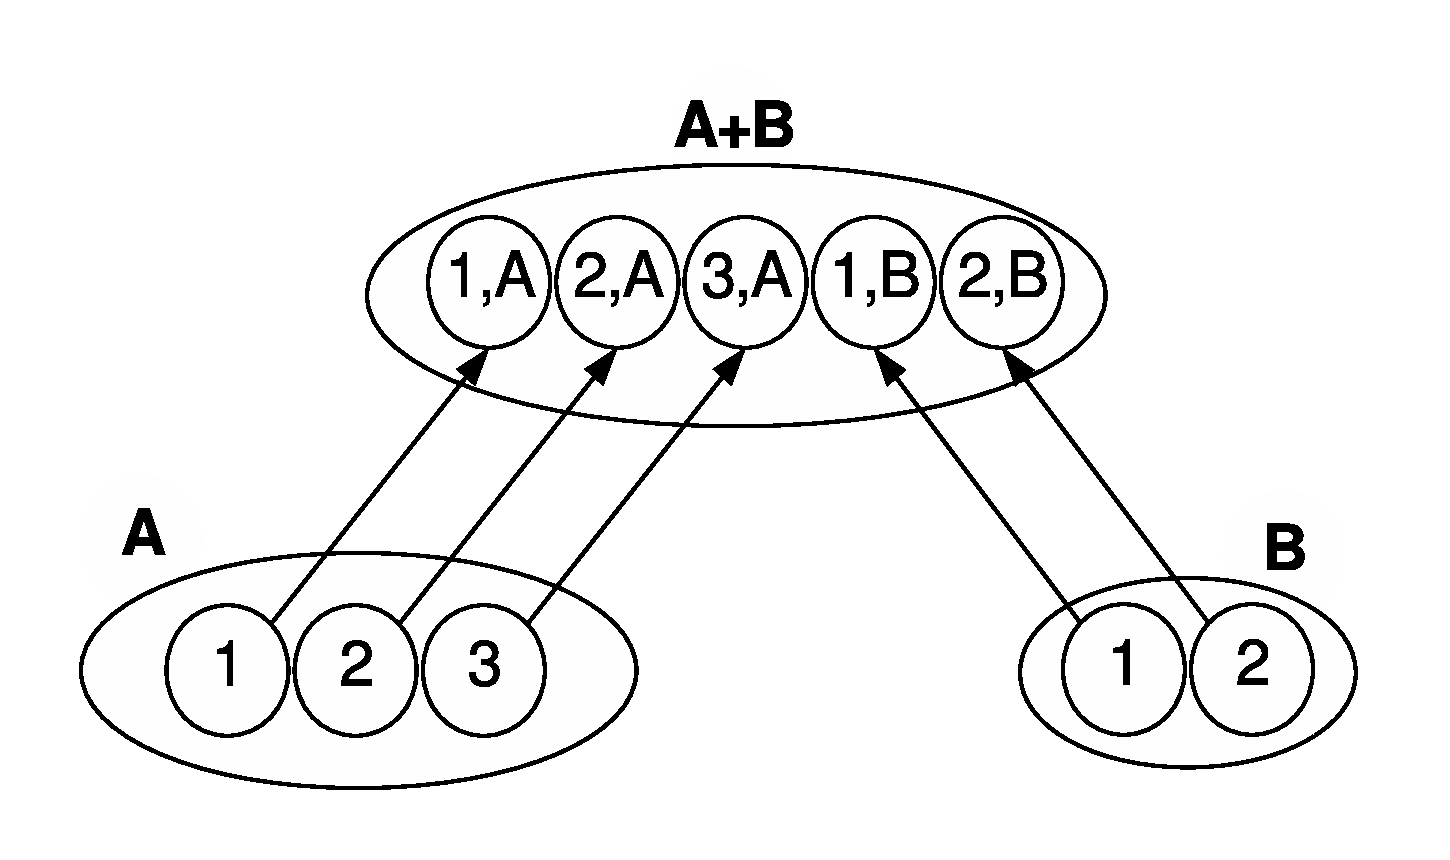
\includegraphics[scale=0.4]{images/gts/coproduct-open}
  \caption{A coproduct in \cat{Set} \important{name the morphisms}}\label{fig:gts:coproduct}
\end{figure}

Notice that $(A+B)' = \{(1,0),(2,0),(3,0),(1,1),(2,1)\}$ or $(A+B)'' = \{a,b,c,d,e\}$ or any other set with five elements would be equally valid as coproducts for this case. This is due to the fact the categories deal with their objects up to isomorphism, i.e. all this objects have the same format regardless of their internal representations.
\end{example}


\begin{definition}[Coequalizer] Given two objects $A$ and $B$ with two parallel morphisms \morph{f}{A}{B} \morph{g}{A}{B}, the coequalizer of the diagram is an object $X$ together with a morphism \morph{h}{B}{X} such that \mbox{$h \circ f = h \circ g$} and, for any other such objects $X'$ with a morphism $h'$, there is a unique morphism \morph{!}{X}{X'} such that the following diagram commutes.

\diagram{
  A\ar@<.5ex>[r]^{f}\ar@<-.5ex>[r]_{g} & B\ar[r]^{h}\ar[dr]_{h'} & X\ar@{.>}[d]^{!}\\
    &   & X'
}
\end{definition}

\begin{example}[Coequalizers in \cat{Set}] Coequalizers generalize the notion of smallest equivalence relation. Figure~\ref{fig:gts:coequalizer} shows the coequalizer for two functions from $A$ to $B$, let $f$ be the one represented with a solid line and $g$ the one with a dashed line. It is easy to see that the function $h$ from $B$ to $X$ corresponds to the equivalence relation that glues together the items that are identified by the functions $f$ and $g$. Notice that $X$ does not contain any other element which is not mapped from $B$ and no element in $X$ was glued together without respecting $f$ and $g$.

\begin{figure}[!ht]
  \centering
  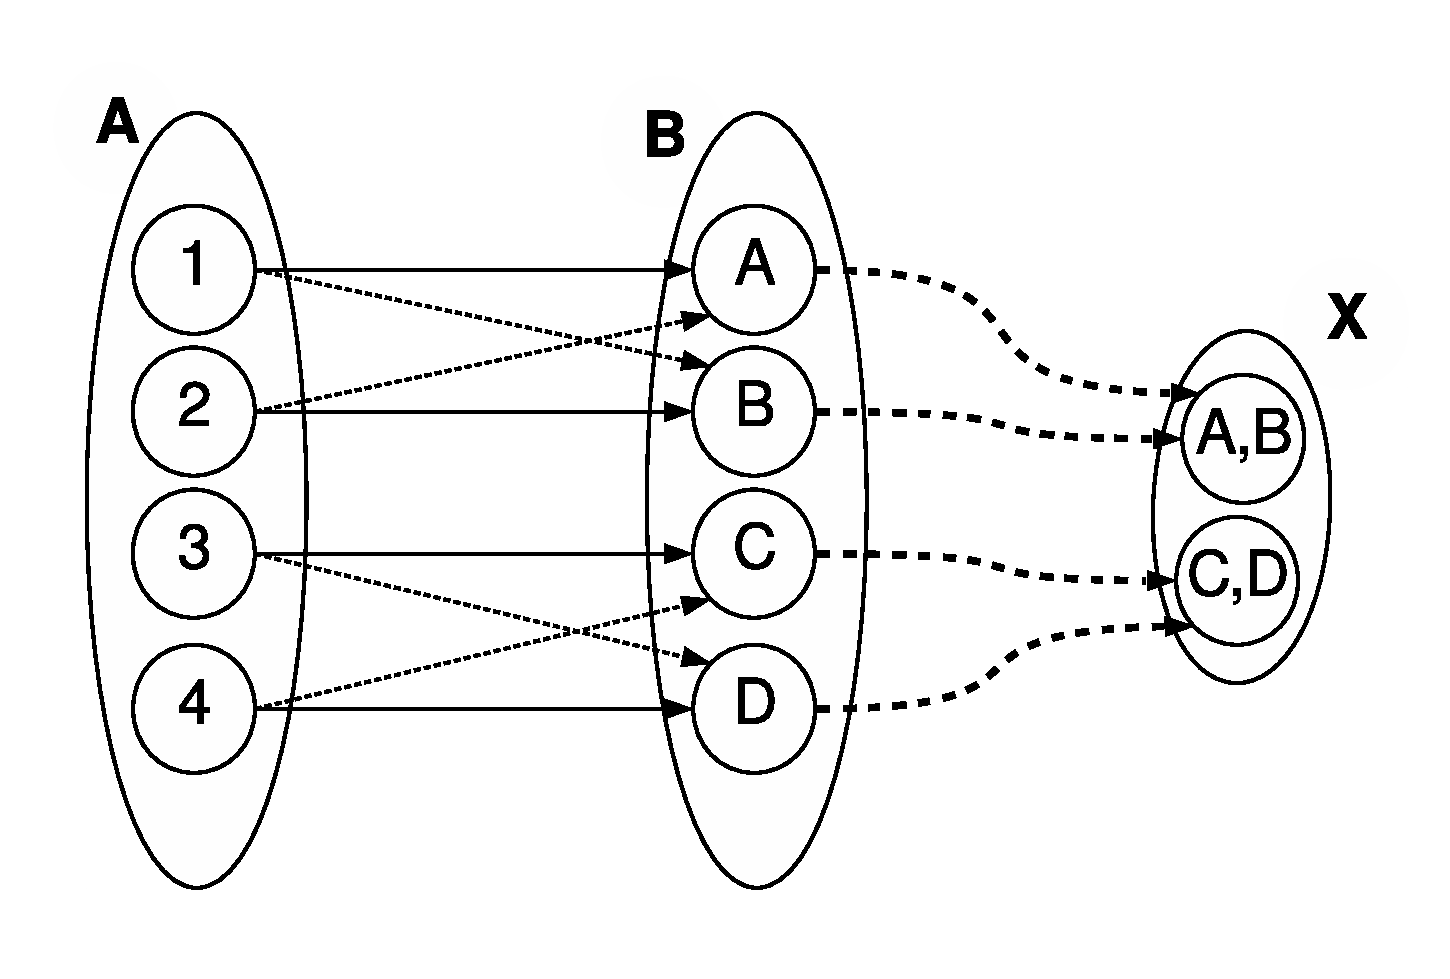
\includegraphics[scale=0.4]{images/gts/coequalizer}
  \caption{A coequalizer in \cat{Set} \important{name the morphism}}\label{fig:gts:coequalizer}
\end{figure}


\end{example}

\begin{definition}[Pushout] Given a span of arrows \mbox{$B \xleftarrow{f} A \xrightarrow{g} C$}, its \emph{pushout} is an object $X$ together with a pair of arrows \morph{f'}{C}{X} and \morph{g'}{B}{X} such that (1) \mbox{$f' \circ g = g' \circ f$} and (2) for any other object $X'$ with morphisms \morph{i}{B}{X'} and \morph{j}{C}{X'} such that $i \circ f = j \circ g$ there is a unique morphism \morph{!}{X}{X'} such that \mbox{$i =$ $! \circ g'$} and \mbox{$j =$ $! \circ f'$}.

\diagram{
  A\ar[r]^{f}\ar[d]_{g} & B\ar[d]^{g'}\ar@/^1.1pc/[rdd]^{i} &\\
  C\ar[r]_{f'}\ar@/_1.1pc/[drr]_{j}       & X\ar@{.>}[dr]^{!}&\\
                &         &X'
}

\end{definition}

\begin{example}[Pushouts in \cat{Set}] A pushout in \cat{Set} can be seen on Figure~\ref{fig:gts:pushout}. Notice that a pushout maps all elements of sets $B$ and $C$ into set $X$, ``gluing'' the ones that are identified via the morphisms \morph{f}{A}{B} and \morph{g}{A}{C}.

\begin{figure}[!ht]
  \centering
  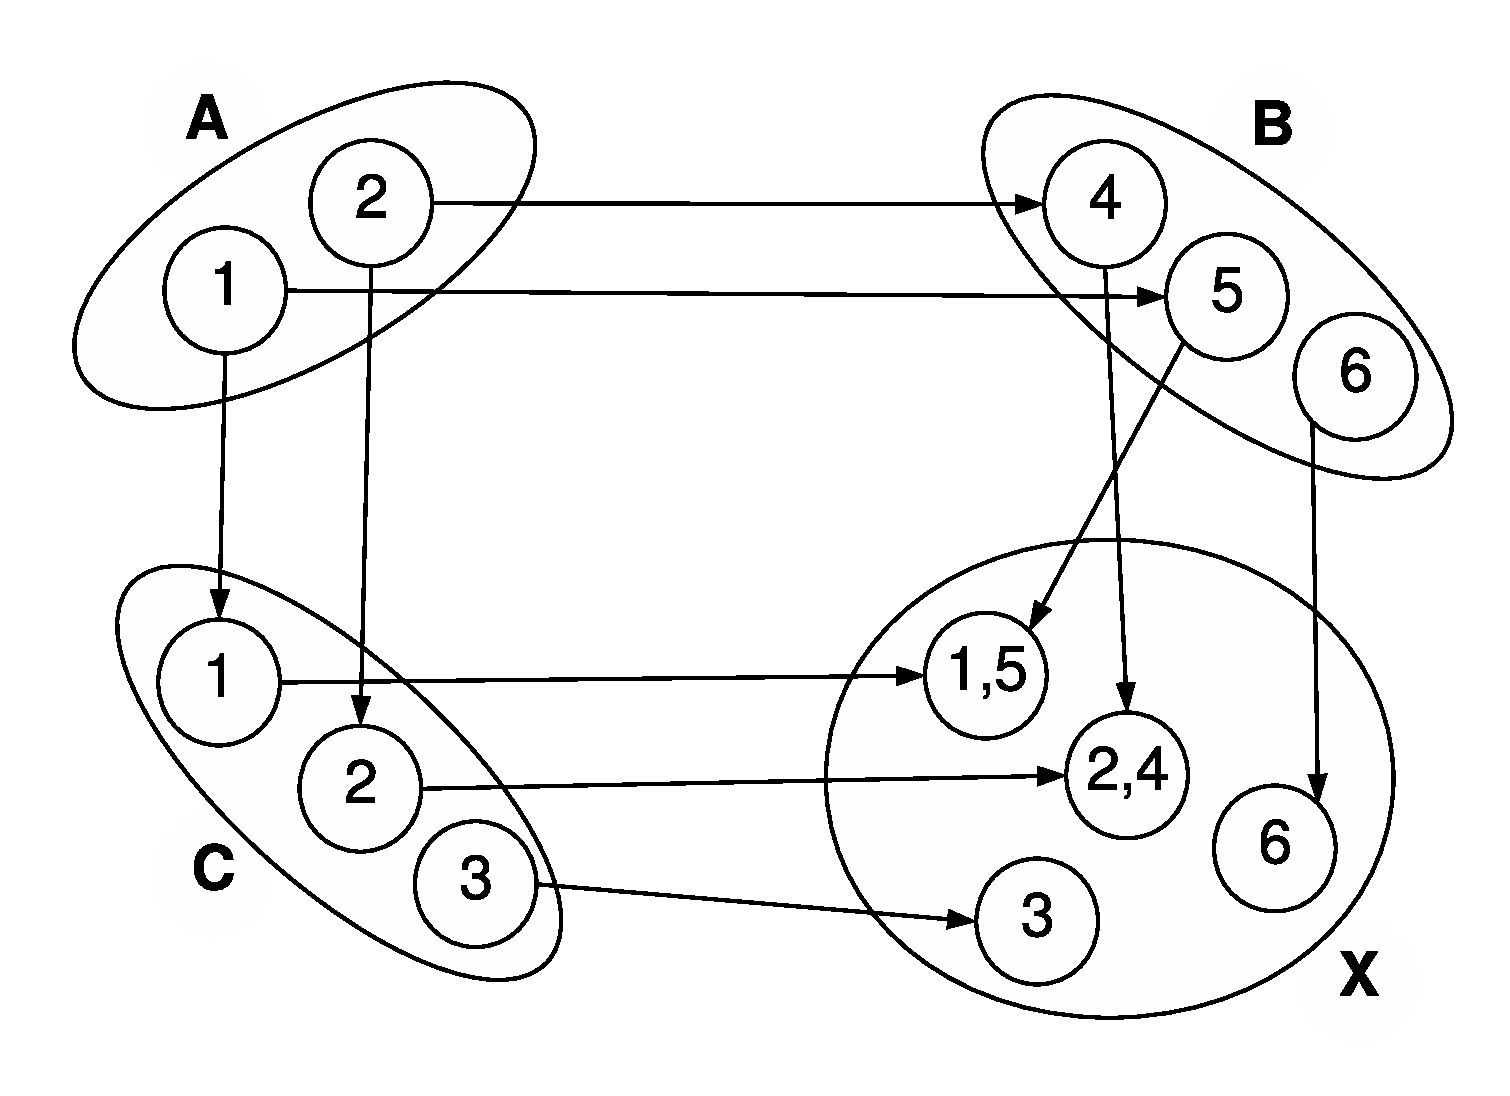
\includegraphics[scale=0.4]{images/gts/pushout}
  \caption{A pushout in \cat{Set} \important{name the morphisms}}\label{fig:gts:pushout}
\end{figure}

\end{example}

\begin{definition}[Colimit] Given a diagram $D$ in a category \cat{C}, a \emph{cocone} for $D$ is an object $X$ and a family of morphisms \morph{f_i}{D_i}{X} (one for each object $D_i$ in $D$), such that for each morphism $g$ in $D$ the outer part of the following diagram commutes.

\diagram{
  D_i\ar[rr]^{g}\ar[dr]_{f_i} &   & D_j\ar[dl]^{f_j}\\
      & X &   \\
}
\hfill

  A \emph{colimit} for a diagram $D$ is a cocone \{\morph{f_i}{D_i}{X}\} such that for any other cocone \{\morph{f'_i}{D'_i}{X'}\} there exists a unique morphism \morph{!}{X}{X'} such that the following diagram commutes for every $D_i$ in $D$.


\diagram{
  D_i\ar@/_1.1pc/[ddr]_{f'_i}\ar[rr]^{g}\ar[dr]_{f_i} &   & D_j\ar@/^1.1pc/[ddl]^{f'_j}\ar[dl]^{f_j}\\
      & X\ar@{.>}[d]^{!} &   \\
      & X'&    \\
}
\end{definition}

\begin{example}[Colimits in \cat{Set}] Colimits generalize several constructions such as disjoint unions, direct sums, coproducts, pushouts and others, where different objects of a diagram are ``glued'' together in one single object respecting commutativity. All previous examples of coproduct, coequalizer and pushout are special cases of colimits. Figure~\ref{fig:gts:colimit} shows a colimit for a diagram that can not be calculated in (one step) by any of the previous constructions.

\begin{figure}[!ht]
  \centering
  \includegraphics[scale=0.4]{images/gts/colimit}
  \caption{A colimit in \cat{Set}}\label{fig:gts:colimit}
\end{figure}

\end{example}


%\chapter{Verigraph Tutorial}\label{app:tutorial}
\includepdf[pages={1-}]{appendix/verigraph-tutorial}

%\chapter{Restaurant System Use Cases}\label{app:use-cases}
\includepdf[pages={1-}]{appendix/use-cases.pdf}

\end{document}
